\begin{dang}{Nhận dạng đồ thị}
\end{dang}
\begin{vd}%[2D1Y5-1]
    \immini
    {
        Cho đồ thị như hình vẽ bên dưới. Hỏi đồ thị là của hàm số nào dưới đây?
        \choice
        {$y=x^3-3x+1$}
        {$y=x^4-3x^2-1$}
        {$y=-x^3-3x-1$}
        {\True $y=x^3-3x-1$}
    }
    {
        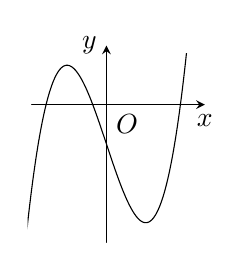
\begin{tikzpicture}[>=stealth,scale=0.5, line join=round, line cap=round]
            \def\a{1} \def\b{0} \def\c{-3} \def\d{-1}
            \def\xt{-1.9} \def\xp{2.5} \def\yt{1.5} \def\yd{-3.5}
            \draw[->] (\xt,0)--(\xp,0) node [below]{$x$};
            \draw[->] (0,\yd)--(0,\yt) node [left]{$y$};
            \node at (0,0) [below right]{$O$};
            \clip (\xt-0.1,\yd+0.1) rectangle (\xp-0.1,\yt-0.2);
            \draw[smooth,samples=300] plot(\x,{\a*(\x)^3+\b*(\x)^2+\c*(\x)+\d});
        \end{tikzpicture}
    }
    \loigiai{
        Từ đồ thị hàm số, ta có hàm số cần tìm là hàm bậc ba có hệ số $a>0$ và hệ số tự do $d<0$ do đó đáp án đúng là $y=x^3-3x-1$.
    }
\end{vd}
\begin{vd}%[2D1Y5-1]
    \immini
    {
        Đồ thị cho ở hình vẽ bên dưới là của hàm số nào trong các hàm số dưới đây?
        \choice
        {$y=-x^3-4$}
        {$y=x^3-3x^2-4$}
        {\True $y=-x^3+3x^2-4$}
        {$y=-x^3+3x^2-2$}
    }
    {
        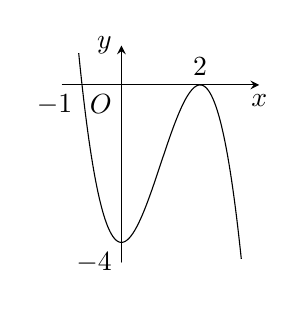
\begin{tikzpicture}[>=stealth,scale=0.5, line join=round, line cap=round]
            \def\a{-1} \def\b{3} \def\c{0} \def\d{-4}
            \def\xt{-1.5} \def\xp{3.5} \def\yt{1} \def\yd{-4.5}
            \draw[->] (\xt,0)--(\xp,0) node [below]{$x$};
            \draw[->] (0,\yd)--(0,\yt) node [left]{$y$};
            \node at (0,0) [below left]{$O$};
            \node at (-1,0) [below left]{$-1$};
            \node at (2,0) [above]{$2$};
            \node at (0,-4) [below left]{$-4$};
            \clip (\xt-0.1,\yd+0.1) rectangle (\xp-0.1,\yt-0.2);
            \draw[smooth,samples=300] plot(\x,{\a*(\x)^3+\b*(\x)^2+\c*(\x)+\d});
        \end{tikzpicture}
    }
    \loigiai{
        Từ đồ thị hàm số, ta thấy hàm số là hàm bậc ba có hệ số $a<0$ và đồ thị cắt trục tung tại điểm có tung độ là $-4$ nên ta loại phương án $y=x^3-3x^2-4$ và $y=-x^3+3x^2-2$.\\
        Ta thấy hàm số cần tìm có hai cực trị, do đó loại phương án $y=-x^3-4$.\\
        Vậy đáp án cần tìm là $y=-x^3+3x^2-4$.
    }
\end{vd}
\begin{vd}%[2D1Y5-1]
    \immini
    {
        Cho đồ thị hàm số có hình vẽ như hình bên dưới. Hỏi đồ thị là của hàm số nào dưới đây?
        \choice
        {\True $y=-x^3+3x+1$}
        {$y=x^3-3x+1$}
        {$y=-x^3+3x^2+1$}
        {$y=-x^3-3x+1$}
    }
    {
        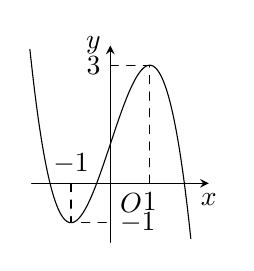
\begin{tikzpicture}[>=stealth,scale=.5, line join=round, line cap=round]
            \def\a{-1} \def\b{0} \def\c{3} \def\d{1}
            \def\xt{-2} \def\xp{2.5} \def\yt{3.5} \def\yd{-1.5}
            \draw[->] (\xt,0)--(\xp,0) node [below]{$x$};
            \draw[->] (0,\yd)--(0,\yt) node [left]{$y$};
            \node at (0,0) [below right]{$O$};	\draw[dashed] (1,0)node[below]{$1$}--(1,3)--(0,3)node[left]{$3$};
            \draw[dashed] (-1,0)node[above]{$-1$}--(-1,-1)--(0,-1)node[right]{$-1$};
            \clip (\xt-0.1,\yd+0.1) rectangle (\xp-0.1,\yt-0.1);
            \draw[smooth,samples=300] plot(\x,{\a*(\x)^3+\b*(\x)^2+\c*(\x)+\d});
        \end{tikzpicture}
    }
    \loigiai{
        \begin{itemize}
            \item Từ đồ thị hàm số ta có hàm số cần tìm là hàm bậc ba có hệ số $a<0$ đo đó loại phương án $y=x^3-3x+1$.
            \item Hàm số cần tìm có $2$ cực trị nên loại phương án $y=-x^3-3x+1$.
            \item Đồ thị hàm số đi qua điểm có tọa độ $(-1;-1)$ nên loại phương án $y=-x^3+3x^2+1$.
        \end{itemize}
        Vậy đáp án cần tìm là $y=-x^3+3x+1$.
    }
\end{vd}
\begin{vd}%[2D1Y5-1]
    \immini
    {
        Bảng biến thiên là của hàm số nào dưới đây?
        \choice
        {$y=\dfrac{x^2-3x-4}{x-2}$}
        {$y=x^3-3x+4$}
        {\True $y=-x^3+3x+2$}
        {$y=\dfrac{x-1}{2x-1}$}
    }
    {
        
\begin{tikzpicture}[>=stealth]
            \tkzTabInit[nocadre=false,lgt=1,espcl=2,deltacl=0.5]{$x$/.7 ,$y'$/.7,$y$/2}
            {$-\infty$ , $-1$ , $1$ , $+\infty$}
            \tkzTabLine{ , - , $0$ , + , $0$ , - , }
            \tkzTabVar{+/$+\infty$ , -/$0$ , +/$4$ , -/$-\infty$}
        \end{tikzpicture}
    }
    \loigiai{
        Dựa vào bảng biến thiên ta thấy hàm số là hàm bậc $3$ với hệ số $a<0$.
    }
\end{vd}
\begin{vd}
    Đồ thị của hàm số $y=x^3-3x-1$ là đường cong nào trong các đường cong sau?
    \choice
    {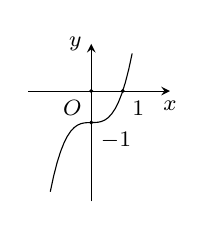
\begin{tikzpicture}[>=stealth, scale=0.4, font=\footnotesize]
            \draw[->] (-2,0)--(2.5,0) node[below] {$x$};
            \draw[->] (0,-3.5)--(0,1.5) node[left] {$y$};
            \draw[domain=-1.3:1.3] plot (\x, {(\x)^3-1});
            \draw[fill=black] (0,0) node[below left=-0.1] {$O$} circle (1.2pt);
            \draw[fill=black] (1,0) node[below right] {$1$} circle (1.2pt);
            \draw[fill=black] (0,-1) node[below right] {$-1$} circle (1.2pt);
    \end{tikzpicture}}
    {\True 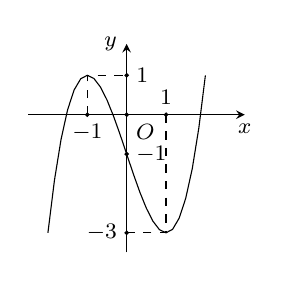
\begin{tikzpicture}[>=stealth, scale=0.5, font=\footnotesize]
            \draw[->] (-2.5,0)--(3,0) node[below] {$x$};
            \draw[->] (0,-3.5)--(0,1.8) node[left] {$y$};
            \draw[domain=-2:2] plot (\x, {(\x)^3-3*\x-1});
            \draw[fill=black] (0,0) node[below right=-0.1] {$O$} circle (1.2pt);
            \draw[fill=black] (1,0) node[above] {$1$} circle (1.2pt);
            \draw[fill=black] (-1,0) node[below] {$-1$} circle (1.2pt);
            \draw[fill=black] (0,-1) node[right] {$-1$} circle (1.2pt);
            \draw[fill=black] (0,1) node[right] {$1$} circle (1.2pt);
            \draw[fill=black] (0,-3) node[left] {$-3$} circle (1.2pt);
            \draw[dashed] (-1,0)--(-1,1)--(0,1) (1,0)--(1,-3)--(0,-3);
    \end{tikzpicture}}
    {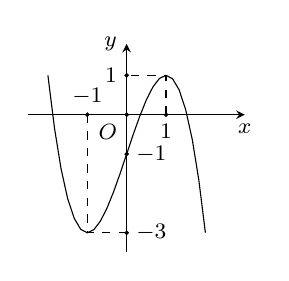
\begin{tikzpicture}[>=stealth, scale=0.5, font=\footnotesize]
            \draw[->] (-2.5,0)--(3,0) node[below] {$x$};
            \draw[->] (0,-3.5)--(0,1.8) node[left] {$y$};
            \draw[domain=-2:2] plot (\x, {-(\x)^3+3*\x-1});
            \draw[fill=black] (0,0) node[below left=-0.1] {$O$} circle (1.2pt);
            \draw[fill=black] (1,0) node[below] {$1$} circle (1.2pt);
            \draw[fill=black] (-1,0) node[above] {$-1$} circle (1.2pt);
            \draw[fill=black] (0,-1) node[right] {$-1$} circle (1.2pt);
            \draw[fill=black] (0,1) node[left] {$1$} circle (1.2pt);
            \draw[fill=black] (0,-3) node[right] {$-3$} circle (1.2pt);
            \draw[dashed] (1,0)--(1,1)--(0,1) (-1,0)--(-1,-3)--(0,-3);
    \end{tikzpicture}}
    {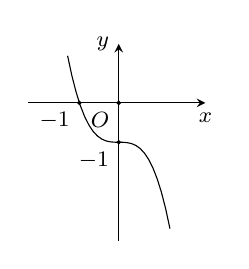
\begin{tikzpicture}[>=stealth, scale=0.5, font=\footnotesize]
            \draw[->] (-2.3,0)--(2.2,0) node[below] {$x$};
            \draw[->] (0,-3.5)--(0,1.5) node[left] {$y$};
            \draw[domain=-1.3:1.3] plot (\x, {-(\x)^3-1});
            \draw[fill=black] (0,0) node[below left=-0.1] {$O$} circle (1.2pt);
            \draw[fill=black] (-1,0) node[below left] {$-1$} circle (1.2pt);
            \draw[fill=black] (0,-1) node[below left] {$-1$} circle (1.2pt);
    \end{tikzpicture}}
    \loigiai{
        Ta có $y'=3x^2-3$. Suy ra $y'=0\Leftrightarrow 3x^2-3=0\Leftrightarrow x=\pm 1$, nên hàm số có hai cực trị là $x=\pm 1$.
        \immini{Ngoài ra hàm số có hệ số $a>0$ nên chọn hình bên
        }{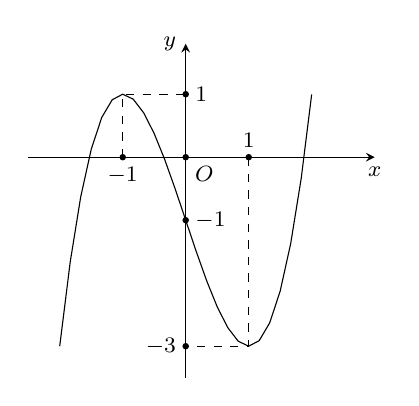
\begin{tikzpicture}[>=stealth, scale=0.8, font=\footnotesize]
                \draw[->] (-2.5,0)--(3,0) node[below] {$x$};
                \draw[->] (0,-3.5)--(0,1.8) node[left] {$y$};
                \draw[domain=-2:2] plot (\x, {(\x)^3-3*\x-1});
                \draw[fill=black] (0,0) node[below right=-0.1] {$O$} circle (1.2pt);
                \draw[fill=black] (1,0) node[above] {$1$} circle (1.2pt);
                \draw[fill=black] (-1,0) node[below] {$-1$} circle (1.2pt);
                \draw[fill=black] (0,-1) node[right] {$-1$} circle (1.2pt);
                \draw[fill=black] (0,1) node[right] {$1$} circle (1.2pt);
                \draw[fill=black] (0,-3) node[left] {$-3$} circle (1.2pt);
                \draw[dashed] (-1,0)--(-1,1)--(0,1) (1,0)--(1,-3)--(0,-3);
        \end{tikzpicture}}
    }
\end{vd}
\begin{vd}
    \immini{
        Đường cong trong hình vẽ bên là đồ thị của hàm số nào dưới đây?
        \choice
        {$y=x^3+x^2+2x+2$}
        {$y=-x^3-4x^2-x+2$}
        {$y=x^3+3x^2-4x+2$}
        {\True $y=x^3+3x^2+4x+2$}
    }{
        \begin{tikzpicture}[>=stealth, scale=0.5, font=\footnotesize]
            \draw[->] (-3,0)--(2,0) node[below] {$x$};
            \draw[->] (0,-3)--(0,3.5) node[left] {$y$};
            \draw[domain=-2.1:0.2] plot(\x, {(\x)^3+3*(\x)^2+4*(\x)+2});
            \draw[fill=black] (0,0) node[below left=-0.1] {$O$} circle (1.2pt);
            \draw[fill=black] (0,2) node[left] {$2$} circle (1.2pt);
            \draw[fill=black] (-1,0) node[above left=0 and -0.1] {$-1$} circle (1.2pt);
            \draw[fill=black] (-2,0) node[above left=0 and -0.1] {$-2$} circle (1.2pt);
            \draw[fill=black] (0,-2) node[right] {$-2$} circle (1.2pt);
            \draw[fill=black] (-2,-2) circle (1.2pt);
            \draw[dashed] (-2,0)--(-2,-2)--(0,-2);
        \end{tikzpicture}
    }
    \loigiai{
        Đây là đồ thị của hàm số bậc ba có hệ số $a>0$ và đi qua các điểm $A(-1;0)$, $B(-2;-2)$.
        Suy ra đây là đồ thị của hàm số $y=x^3+3x^2+4x+2$.
    }
\end{vd}
\begin{vd}%[2D1K5-1]
    \immini
    {
        Cho đồ thị hàm số $y=ax^3+bx^2+cx+d$ như hình vẽ. tìm mệnh đề {\bf đúng}?
        \choice
        {$a>0$, $d>0$, $b<0$, $c<0$}
        {\True $a<0$, $b<0$, $c<0$, $d>0$}
        {$a>0$, $c>0$, $d>0$, $b<0$}
        {$a<0$, $b>0$, $c<0$, $d>0$}
    }
    {
        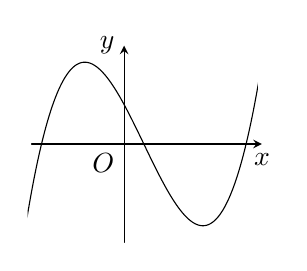
\begin{tikzpicture}[>=stealth,scale=.5, line join=round, line cap=round]
            \def\a{4/13} \def\b{-6/13} \def\c{-24/13}
            \def\d{1}
            \def\xt{-2.35} \def\xp{3.5} \def\yt{2.5} \def\yd{-2.5}
            \draw[->] (\xt,0)--(\xp,0) node [below]{$x$};
            \draw[->] (0,\yd)--(0,\yt) node [left]{$y$};
            \node at (0,0) [below left]{$O$};
            \clip (\xt-0.1,\yd+0.1) rectangle (\xp-0.1,\yt-0.1);
            \draw[smooth,samples=300] plot(\x,{\a*(\x)^3+\b*(\x)^2+\c*(\x)+\d});
        \end{tikzpicture}
    }
    \loigiai{
        Từ đồ thị hàm số, ta thấy $a<0,d>0$ nên đáp án đúng là $a<0,b<0,c<0,d>0$.
    }
\end{vd}
\begin{vd}%[2D1K5-1]
    \immini
    {
        Cho đồ thị hàm số $y=ax^3+bx^2+cx+d$ như hình vẽ bên dưới. Tìm mệnh đề {\bf đúng}?
        \choice
        {$a<0, b>0, c>0, d>0$}
        {$a<0, b<0, c=0, d>0$}
        {$a>0, b<0, c>0, d>0$}
        {\True $a<0, b>0, c=0, d>0$}
    }
    {
        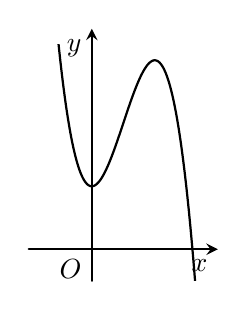
\begin{tikzpicture}[line join=round, line cap=round,>=stealth,thick, scale=0.8]
            \tikzset{label style/.style={font=\footnotesize}}
            \draw[->] (-1,0)--(2,0) node[below left] {$x$};
            \draw[->] (0,-0.5)--(0,3.5) node[below left] {$y$};
            \draw (0,0) node [below left] {$O$};
            \begin{scope}
                \clip (-1,-0.5) rectangle (2,3.25);
                \draw[samples=200,domain=-1:2,smooth,variable=\x] plot (\x,{-4*((\x)^3)+6*((\x)^2)+0*(\x)+1});
            \end{scope}
        \end{tikzpicture}
    }
    \loigiai{
        Từ đồ thị ta thấy đáp án đúng là	$a<0, b>0, c=0, d>0$.
    }
\end{vd}
\begin{vd}
    Đường cong nào dưới đây là đồ thị của hàm số $y=\dfrac{1-x}{x+1}$?
    \choice
    {\begin{tikzpicture}[>=stealth, scale=0.4, font=\footnotesize]
            \draw[->] (-5,0)--(4,0) node[below] {$x$};
            \draw[->] (0,-3)--(0,5) node[left] {$y$};
            \draw[domain=-0.5:3.5] plot(\x, {(\x-1)/(\x+1)});
            \draw[domain=-4.5:-1.6] plot(\x, {(\x-1)/(\x+1)});
            \draw (-5,1)--(3.7,1) (-1,-3)--(-1,4.8);
            \draw[fill=black] (0,0) node[below left=-0.1] {$O$} circle (1.2pt);
            \draw[fill=black] (0,1) node[above right] {$1$} circle (1.2pt);
            \draw[fill=black] (-1,0) node[below left=0 and -0.1] {$-1$} circle (1.2pt);
            \draw[fill=black] (1,0) node[above left=0 and -0.1] {$1$} circle (1.2pt);
            \draw[fill=black] (0,-1) node[right] {$-1$} circle (1.2pt);
    \end{tikzpicture}}
    {\True \begin{tikzpicture}[>=stealth, scale=0.4, font=\footnotesize]
            \draw[->] (-5,0)--(4,0) node[below] {$x$};
            \draw[->] (0,-5)--(0,3) node[left] {$y$};
            \draw[domain=-0.5:3.5] plot(\x, {(\x-1)/(-\x-1)});
            \draw[domain=-4.5:-1.6] plot(\x, {(\x-1)/(-\x-1)});
            \draw (-5,-1)--(3.7,-1) (-1,-5)--(-1,2.8);
            \draw[fill=black] (0,0) node[below left=-0.1] {$O$} circle (1.2pt);
            \draw[fill=black] (0,1) node[above right] {$1$} circle (1.2pt);
            \draw[fill=black] (-1,0) node[above left=0 and -0.1] {$-1$} circle (1.2pt);
            \draw[fill=black] (1,0) node[above right=0 and -0.1] {$1$} circle (1.2pt);
            \draw[fill=black] (0,-1) node[below right] {$-1$} circle (1.2pt);
    \end{tikzpicture}}
    {\begin{tikzpicture}[>=stealth, scale=0.4, font=\footnotesize]
            \draw[->] (-5,0)--(4,0) node[below] {$x$};
            \draw[->] (0,-3)--(0,6.2) node[left] {$y$};
            \draw[domain=-0.4:3.5] plot(\x, {(2*\x-1)/(\x+1)});
            \draw[domain=-4.5:-1.8] plot(\x, {(2*\x-1)/(\x+1)});
            \draw (-5,2)--(3.7,2) (-1,-3)--(-1,6);
            \draw[fill=black] (0,0) node[below left=-0.1] {$O$} circle (1.2pt);
            \draw[fill=black] (0,2) node[above right] {$2$} circle (1.2pt);
            \draw[fill=black] (-1,0) node[below left=0 and -0.1] {$-1$} circle (1.2pt);
            \draw[fill=black] (0,-1) node[right] {$-1$} circle (1.2pt);
    \end{tikzpicture}}
    {\begin{tikzpicture}[>=stealth, scale=0.4, font=\footnotesize]
            \draw[->] (-3,0)--(6,0) node[below] {$x$};
            \draw[->] (0,-5)--(0,4.2) node[left] {$y$};
            \draw[domain=2.3:5.5] plot(\x, {(\x-1)/(-\x+2)});
            \draw[domain=-3:1.8] plot(\x, {(\x-1)/(-\x+2)});
            \draw (-3,-1)--(5.7,-1) (2,-5)--(2,4);
            \draw[fill=black] (0,0) node[below left=-0.1] {$O$} circle (1.2pt);
            \draw[fill=black] (2,0) node[above right=0 and -0.1] {$2$} circle (1.2pt);
            \draw[fill=black] (1,0) node[above left=0 and -0.1] {$1$} circle (1.2pt);
            \draw[fill=black] (0,-1) node[below left] {$-1$} circle (1.2pt);
    \end{tikzpicture}}
    \loigiai{
        Đồ thị của hàm số đã cho có tiệm cận đứng $x=-1$, tiệm cận ngang $y=-1$. Ngoài ra đồ thị hàm số còn qua các điểm $A(1;0)$ và $B(0;1)$. \immini{Đồ thị ở phương án thỏa mãn các tính chất trên.
        }{
            \begin{tikzpicture}[>=stealth, scale=0.4, font=\footnotesize]
                \draw[->] (-5,0)--(4,0) node[below] {$x$};
                \draw[->] (0,-5)--(0,3) node[left] {$y$};
                \draw[domain=-0.5:3.5] plot(\x, {(\x-1)/(-\x-1)});
                \draw[domain=-4.5:-1.6] plot(\x, {(\x-1)/(-\x-1)});
                \draw (-5,-1)--(3.7,-1) (-1,-5)--(-1,2.8);
                \draw[fill=black] (0,0) node[below left=-0.1] {$O$} circle (1.2pt);
                \draw[fill=black] (0,1) node[above right] {$1$} circle (1.2pt);
                \draw[fill=black] (-1,0) node[above left=0 and -0.1] {$-1$} circle (1.2pt);
                \draw[fill=black] (1,0) node[above right=0 and -0.1] {$1$} circle (1.2pt);
                \draw[fill=black] (0,-1) node[below right] {$-1$} circle (1.2pt);
            \end{tikzpicture}
        }
    }
\end{vd}
\begin{vd}%[2D1Y5-1]
    \immini
    {
        Trong 4 hàm số sau hàm số nào có bảng biến thiên như hình vẽ?
        \choice
        {$y=\dfrac{x-1}{x+2}$}
        {$y=\dfrac{2x+1}{x-1}$}
        {$y=\dfrac{x-4}{x-2}$}
        {\True $y=\dfrac{x+1}{x-2}$}
    }
    {
        
\begin{tikzpicture}
            \tikzset{double style/.append style={double distance=1.5pt}}
            \tkzTabInit[nocadre=false,lgt=1.5,espcl=3,deltacl=0.6]
            {$x$ /0.75,$f'(x)$ /0.75,$f(x)$ /1.7}
            {$-\infty$,$2$,$+\infty$}
            \tkzTabLine{,-,d,-,}
            \tkzTabVar{+/$1$,-D+/$-\infty$/$+\infty$,-/$1$}
        \end{tikzpicture}
    }
    \loigiai{
        Dựa vào bảng biến thiên ta có: phương trình tiệm cận đứng là $x=2$, tiệm cận ngang là $y=1$.\\
        (Loại được đáp án A, B).\\
        Hàm số nghịch biến trên $(-\infty; 2)$ và $(2;+\infty)$ nên C sai vì $y'=\dfrac{2}{(x-2)^2}>0$.\\
        Chọn phương án D vì có đạo hàm $y'=\dfrac{-3}{(x-2)^2}<0\forall x\in \mathscr{D}$.}
\end{vd}
\begin{vd}%[2D1Y5-1]
    \immini
    {Hình vẽ sau đây là hình dạng đồ thị của hàm số nào
        \choice
        {$y=\dfrac{x+2}{x+1}$}
        {\True $y=\dfrac{x+2}{x-1}$}
        {$y=\dfrac{x-2}{x-1}$}
        {$y=\dfrac{x}{x-1}$}}
    {\begin{tikzpicture}[>=stealth,x=1cm,y=1cm,scale=0.4]
            \def\a{1}
            \def\b{2}
            \def\c{1}
            \def\d{-1}
            \draw[->] (-4,0) -- (6,0) node[below] {\scriptsize $x$};
            \draw[->] (0,-4) -- (0,6) node[left] {\scriptsize $y$};
            \draw (0,0)node[below left]{\scriptsize $O$};
            \fill (1,0)node[below right]{\scriptsize $1$}circle(1.5pt);
            \fill (0,1)node[above left]{\scriptsize $1$}circle(1.5pt);
            \draw[dashed,blue] (1,-4)--(1,6) (-4,1)--(6,1);
            \clip (-4,-4)rectangle(6,6);
            \pgfmathsetmacro{\can}{-(\d)/(\c)}
            \draw[thick,samples=150,smooth,domain=-4:{\can-.1}] plot(\x,{(\a*\x+(\b))/(\c*\x+(\d))});
            \draw[thick,samples=150,smooth,domain={\can+.1}:6] plot(\x,{(\a*\x+(\b))/(\c*\x+(\d))});
    \end{tikzpicture}}
    \loigiai{
        Dựa vào đồ thị ta thấy hàm số luôn nghịch biến trên từng khoảng xác định và có phương trình hai đường tiệm cận là $x=1$ và $y=1$ và cắt trục tung tại điểm có tọa độ $(0;-2)$ nên hàm số phải là $y=\dfrac{x+2}{x-1}$.}
\end{vd}
\begin{vd}%[2D1Y5-1]
    \immini
    {Đường cong trong hình bên là đồ thị của một hàm số trong bốn hàm số dưới đây. Hỏi hàm số đó là hàm số nào?
        \choice
        {$y=\dfrac{2x+1}{2x-2}$}
        {$y=\dfrac{-x}{1-x}$}
        {$y=\dfrac{x-1}{x+1}$}
        {\True $y=\dfrac{x+1}{x-1}$}}
    {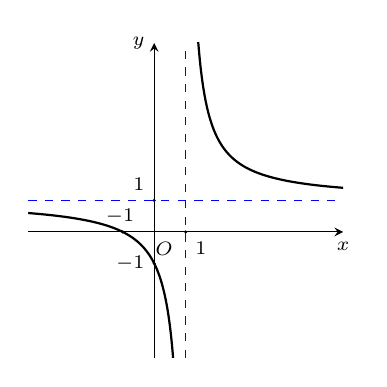
\begin{tikzpicture}[>=stealth,x=1cm,y=1cm,scale=0.4]
            \def\a{1}
            \def\b{1}
            \def\c{1}
            \def\d{-1}
            \draw[->] (-4,0) -- (6,0) node[below] {\scriptsize $x$};
            \draw[->] (0,-4) -- (0,6) node[left] {\scriptsize $y$};
            \draw (0,0)node[shift={(300:2.5mm)}]{\scriptsize $O$};
            \fill (1,0)node[below right]{\scriptsize $1$}circle(1.5pt);
            \fill (0,1)node[above left]{\scriptsize $1$}circle(1.5pt);
            \fill (-1,0)node[shift={(100:2mm)}]{\scriptsize $-1$}circle(1.5pt);
            \fill (0,-1)node[left]{\scriptsize $-1$}circle(1.5pt);
            \draw[dashed,blue] (1,-4)--(1,6) (-4,1)--(6,1);
            \clip (-4,-4)rectangle(6,6);
            \pgfmathsetmacro{\can}{-(\d)/(\c)}
            \draw[thick,samples=150,smooth,domain=-4:{\can-.1}] plot(\x,{(\a*\x+(\b))/(\c*\x+(\d))});
            \draw[thick,samples=150,smooth,domain={\can+.1}:6] plot(\x,{(\a*\x+(\b))/(\c*\x+(\d))});
    \end{tikzpicture}}
    \loigiai{
        Từ hình vẽ suy ra đồ thị hàm số có tiệm cận ngang là $y=1$ và tiệm cận đứng là $x=1$ đồng thời đồ thị đi qua điểm $(0;-1)$ nên hàm số $y=\dfrac{x+1}{x-1}$ thỏa mãn.}
\end{vd}
\begin{vd}%[2D1Y5-1]
    \immini{
        Giá trị $a, b$ để hàm số $y=\dfrac{ax+b}{x-1}$ có đồ thị như hình bên là
        \choice
        {$a=-1,b=2$}
        {$a=-1,b=-2$}
        {\True $a=1,b=2$}
        {$a=-1,b=-2$}
    }{
        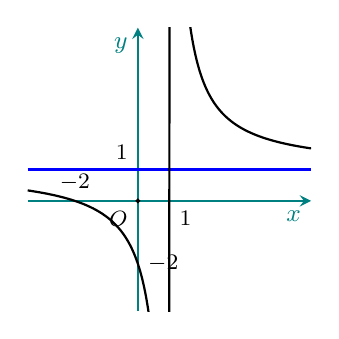
\begin{tikzpicture}[thick,>=stealth,scale=0.4]
            \clip(-3.5,-3.5) rectangle (5.5,5.5);
            \draw[->,teal] (-3.5,0) -- (5.5,0) node[below left] {\small $x$};
            \draw[->,teal] (0,-3.5) -- (0,5.5) node[below left] {\small $y$};
            \draw[blue] (-3.5,1.0) -- (5.5,1.0);
            \draw [fill=white,draw=black] (0,0) circle (1pt)node[below left] {\footnotesize $O$};
            \draw(1.0,0) node[below right] {\footnotesize $1$};
            \draw (-2,0) node[above] {\footnotesize $-2$};
            \draw (0,-2) node[right] {\footnotesize $-2$};
            \draw (0,1.0) node[above left] {\footnotesize $1$};
            \draw[thick,black,smooth,samples=100,domain=-3.5:5.5] plot(\x,{(\x+2)/(\x-1)});
        \end{tikzpicture}
    }
    \loigiai{
        Ta có đồ thị hàm số $y=\dfrac{ax+b}{x-1}$ có tiệm cận ngang $y=a\Rightarrow a=1$, đồ thị hàm số cắt trục tung tại điểm có tọa độ $(0;-b)\Rightarrow b=2$.}
\end{vd}
\begin{vd}
    \immini{
        Đường cong trong hình bên là đồ thị của hàm số nào dưới đây?
        \choice
        {\True $y=\dfrac{x^2+2x+2}{-x-1}$}
        {$y=\dfrac{x^2+2x+2}{x+1}$}
        {$y=\dfrac{x^2-2x+2}{x-1}$}
        {$y=\dfrac{x^2-2x+2}{x+1}$}
    }{
        \begin{tikzpicture}[>=stealth, scale=0.4, font=\footnotesize]
            \draw[->] (-5.3,0)--(4.5,0) node[below] {$x$};
            \draw[->] (0,-5.5)--(0,6) node[left] {$y$};
            \draw[domain=-0.8:3] plot(\x, {((\x)^2+2*(\x)+2)/(-\x-1)});
            \draw[domain=-4.5:-1.2] plot(\x, {((\x)^2+2*(\x)+2)/(-\x-1)});
            \draw[fill=black] (0,0) node[above right=-0.1] {$O$} circle (1.2pt);
            \draw (-1,-5.4)--(-1,5.6);
            \draw[fill=black] (-1,0) node[below left=0 and -0.1] {$-1$} circle (1.2pt);
            \draw[fill=black] (0,-1) node[above right=-0.1] {$-1$} circle (1.2pt);
            \draw[fill=black] (0,-2) node[above left=-0.1] {$-2$} circle (1.2pt);
            \draw[domain=-5:3.7] plot(\x, {-\x-1});
        \end{tikzpicture}
    }
    \loigiai{
        Đồ thị có tiệm cận đứng $x=-1$ và đi qua điểm $A(0;-2)$, suy ra hàm số cần tìm là $y=\dfrac{x^2+2x+2}{-x-1}$.
    }
\end{vd}
\begin{vd}%[2D1H5-1]
    Đồ thị trong hình vẽ bên dưới là đồ thị của hàm số nào?
    \begin{center}
        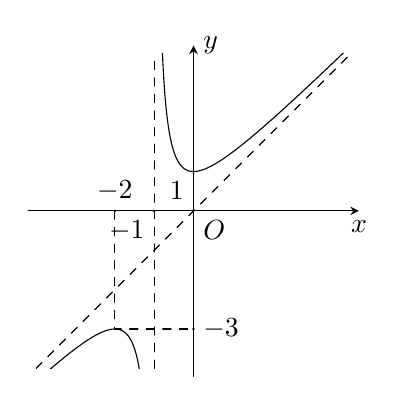
\begin{tikzpicture}[scale=0.5, line join=round, line cap=round, >=stealth]
            \tikzset{every node/.style={scale=1}}
            \def\xmin{-4}\def\xmax{4}\def\ymin{-4}\def\ymax{4}
            \draw[->] (\xmin-0.2,0)--(\xmax+0.2,0) node[below]{$x$};
            \draw[->] (0,\ymin-0.2)--(0,\ymax+0.2) node[right]{$y$};
            \draw (0,0) node[below right]{$O$};
            % \foreach \x in {-3,-2,-1,1,2,3}\draw (\x,0.1)--(\x,-0.1) node[below]{$\x$};
            % \foreach \y in {-3,-2,-1,1,2,3}\draw (0.1,\y)--(-0.1,\y) node[left]{$\y$};
            \clip (\xmin,\ymin) rectangle (\xmax,\ymax);
            \draw[dashed] (-1.0,\ymin)--(-1.0,\ymax);
            \draw[dashed,domain=\xmin:\xmax] plot (\x,{1.0*(\x)+0.0});
            \draw[smooth,samples=200,domain=\xmin:-1.1] plot (\x,{(1*((\x)^2)+1*(\x)+1)/(1*(\x)+1)});
            \draw[smooth,samples=200,domain=-0.9:\xmax] plot (\x,{(1*((\x)^2)+1*(\x)+1)/(1*(\x)+1)});
            \fill (-2,0) circle(1pt) node[above]{$-2$};
            \fill (-1,0) circle(1pt) node[below left]{$-1$};
            \fill (0,-3) circle(1pt) node[right]{$-3$};
            \fill (0,1) circle(1pt) node[below left]{$1$};
            \draw[dashed] (-2, 0) -- (-2, -3) -- (0, -3);
        \end{tikzpicture}
    \end{center}
    \choice
    {$y=x-\dfrac{1}{x+1}$}
    {$y=\dfrac{2x+1}{x+1}$}
    {$y=\dfrac{x^2-x+1}{x+1}$}
    {\True $y=\dfrac{x^2+x+1}{x+1}$}
    \loigiai{
        Đồ thị hàm số có tiệm cận xiên nên loại hàm số $y=\dfrac{2x+1}{x+1}$.\\
        Đồ thị hàm số cắt trục tung tại điểm $\left(0;1 \right)$ nên loại hàm số $y=x-\dfrac{1}{x+1}$.\\
        Đồ thị hàm số đi qua điểm $\left(-2;-3 \right)$ nên loại hàm số $y=\dfrac{x^2-x+1}{x+1}$.
    }
\end{vd}
\BTTN
\Opensolutionfile{ans}[ans/2D1-5-DANG-1]
\begin{ex}%[2D1Y5-1]
    \immini
    {
        Cho đồ thị như hình vẽ bên dưới. Hỏi đồ thị là của hàm số nào dưới đây?
        \choice
        {$y=-x^2+x-1$}
        {$y=-x^3+3x+1$}
        {$y=x^4-x^2+1$}
        {\True $y=x^3-3x+1$}
    }
    {
        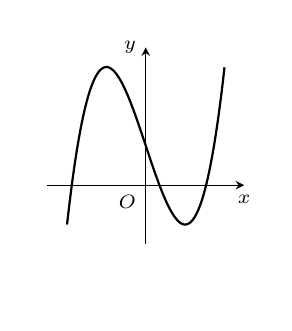
\begin{tikzpicture}[>=stealth,x=1cm,y=1cm,scale=0.5]
            \def\a{1}
            \def\b{0}
            \def\c{-3}
            \def\d{1}
            \draw[->] (-2.5,0) -- (2.5,0)node[below]{\scriptsize $x$};
            \draw[->] (0,-1.5) -- (0,3.5) node[left] {\scriptsize $y$};
            \draw (0,0)node[below left]{\scriptsize $O$};
            \clip (-3,-3)rectangle(3,4);
            \draw[thick,samples=150,smooth,domain=-2:2] plot(\x,{\a*(\x)^3+(\b)*(\x)^2+(\c)*\x+(\d)});
        \end{tikzpicture}
    }
    \loigiai{
        Dựa vào đồ thị hàm số ta thấy hàm số là hàm bậc $3$ có hệ số $a>0$, do đó đáp án là $y=x^3-3x+1$.
    }
\end{ex}
\begin{ex}%[2D1Y5-1]
    \immini
    {
        Đồ thị trong hình vẽ bên dưới là của hàm số nào dưới đây?
        \choice
        {$y=x^3+3x^3-3x+1$}
        {$y=-x^3-2x^2+x-2$}
        {\True $y=-x^3+3x+1$}
        {$y=x^3+3x^2+3x+1$}
    }
    {
        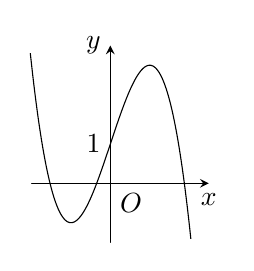
\begin{tikzpicture}[>=stealth,scale=0.5, line join=round, line cap=round]
            \def\a{-1} \def\b{0} \def\c{3} \def\d{1}
            \def\xt{-2} \def\xp{2.5} \def\yt{3.5} \def\yd{-1.5}
            \draw[->] (\xt,0)--(\xp,0) node [below]{$x$};
            \draw[->] (0,\yd)--(0,\yt) node [left]{$y$};
            \node at (0,0) [below right]{$O$};
            \node at (0,1) [left]{$1$};
            \clip (\xt-0.1,\yd+0.1) rectangle (\xp-0.1,\yt-0.2);
            \draw[smooth,samples=300] plot(\x,{\a*(\x)^3+\b*(\x)^2+\c*(\x)+\d});
        \end{tikzpicture}
    }
    \loigiai{
        Từ đồ thị hàm số, ta có hàm cần tìm là hàm bậc ba có hệ số $a<0$. Đồ thị hàm số cắt trục $Oy$ tại điểm có tung độ bằng $1$ nên hệ số tự do $d=1$. Vậy đáp án cần tìm là $y=-x^3+3x+1$.
    }
\end{ex}
\begin{ex}%[2D1Y5-1]
    \immini
    {
        Hình vẽ bên dưới là của hàm số nào trong các hàm số dưới đây?
        \choice
        {$y=x^3-3x^2$}
        {$y-x^4+2x^2$}
        {$y=1+3x-x^3$}
        {\True $y=3x-x^3$}
    }
    {
        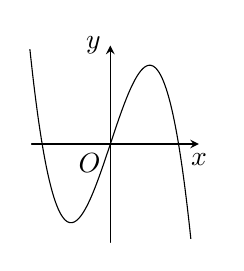
\begin{tikzpicture}[>=stealth,scale=0.5, line join=round, line cap=round]
            \def\a{-1} \def\b{0} \def\c{3} \def\d{0}
            \def\xt{-2} \def\xp{2.25} \def\yt{2.5} \def\yd{-2.5}
            \draw[->] (\xt,0)--(\xp,0) node [below]{$x$};
            \draw[->] (0,\yd)--(0,\yt) node [left]{$y$};
            \node at (0,0) [below left]{$O$};
            \clip (\xt-0.1,\yd+0.1) rectangle (\xp-0.1,\yt-0.1);
            \draw[smooth,samples=300] plot(\x,{\a*(\x)^3+\b*(\x)^2+\c*(\x)+\d});
        \end{tikzpicture}
    }
    \loigiai{
        Từ đồ thị hàm số ta thấy hàm số cần tìm là hàm bậc ba có hệ số $a<0$ và đồ thị hàm số đi qua gốc tọa độ $O(0;0)$ nên có hệ số $d=0$. Do đó đáp án đúng là $y=3x-x^3$.
    }
\end{ex}
\begin{ex}%[2D1Y5-1]
    \immini
    {
        Cho đồ thị hàm số $y=ax^3+bx^2+cx+d$. Tìm mệnh đề {\bf đúng} trong các mệnh đề sau?
        \choice
        {$y'>0, \forall x\in \mathbb{R}$}
        {$y'<0,\forall x\in \mathbb{R}$}
        {$y'>0, \forall x>1$}
        {\True $y'>0, \forall x<1$}
    }
    {
        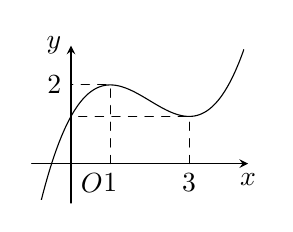
\begin{tikzpicture}[>=stealth,scale=0.5, line join=round, line cap=round]
            \def\a{1} \def\b{-6} \def\c{9} \def\d{6}
            \def\xt{-1} \def\xp{4.5} \def\yt{3} \def\yd{-1}
            \draw[->] (\xt,0)--(\xp,0) node [below]{$x$};
            \draw[->] (0,\yd)--(0,\yt) node [left]{$y$};
            \node at (0,0) [below right]{$O$};
            \draw[dashed] (1,0)node[below]{$1$}--(1,2)--(0,2)node[left]{$2$};
            \draw[dashed] (3,0)node[below]{$3$}--(3,1.2)--(0,1.2);
            \clip (\xt-0.1,\yd+0.1) rectangle (\xp-0.1,\yt-0.1);
            \draw[smooth,samples=300] plot(\x,{\a*(\x)^3/5+\b*(\x)^2/5+\c*(\x)/5+\d/5});
        \end{tikzpicture}
    }
    \loigiai{
        Từ đồ thị hàm số ta thấy hàm số đồng biến trên các khoảng $(-\infty; 1)$ và $(3;+\infty)$; hàm số nghịch biến trên các khoảng $(1;3)$.\\
        Do đó ta có $y'>0, \forall x\in (-\infty;1)\cup (3;+\infty)$ và $y'<0, \forall x \in (1;3)$.\\
        Do đó đáp án đúng là $y'>0, \forall x<1$.
    }
\end{ex}
\begin{ex}%[2D1Y5-1]
    \immini
    {
        Cho đồ thị hàm số $y=ax^3+bx^2+cx+d$. Tìm mệnh đề {\bf đúng} trong các mệnh đề sau?
        \choice
        {$y', \forall x\in \mathbb{R}$}
        {$y'<0, \forall x\in \mathbb{R}$}
        {\True $y'\geq 0, \forall x\in \mathbb{R}$}
        {$y'\leq 0, \forall x\in \mathbb{R}$}
    }
    {
        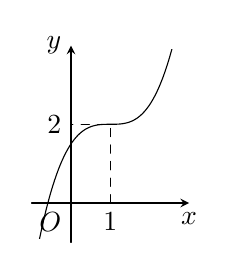
\begin{tikzpicture}[>=stealth,scale=0.5, line join=round, line cap=round]
            \def\a{0.5} \def\b{-1.5} \def\c{1.5} \def\d{1.5} % Hệ số
            \def\xt{-1} \def\xp{3} \def\yt{4} \def\yd{-1}
            \draw[->] (\xt,0)--(\xp,0) node [below]{$x$};
            \draw[->] (0,\yd)--(0,\yt) node [left]{$y$};
            \node at (0,0) [below left]{$O$};
            \draw[dashed] (1,0)node[below]{$1$}--(1,2)--(0,2)node[left]{$2$};
            \clip (\xt-0.1,\yd+0.1) rectangle (\xp-0.1,\yt-0.1);
            \draw[smooth,samples=300] plot(\x,{\a*(\x)^3+\b*(\x)^2+\c*(\x)+\d});
        \end{tikzpicture}
    }
    \loigiai{
        Từ đồ thị ta có đáp án đúng là $y'\geq 0, \forall x\in \mathbb{R}$.
    }
\end{ex}
\begin{ex}%[2D1Y5-1]
    \immini
    {
        Cho đồ thị hàm số $y=ax^3+bx^2+cx+d$. Tìm mệnh đề {\bf đúng} trong các mệnh đề sau?
        \choice
        {$y'>0, \forall x<2$}
        {$y'=0, \forall x<2$}
        {$y'\geq 0, \forall x\in \mathbb{R}$}
        {\True $y'\leq 0, \forall x\in \mathbb{R}$}
    }
    {
        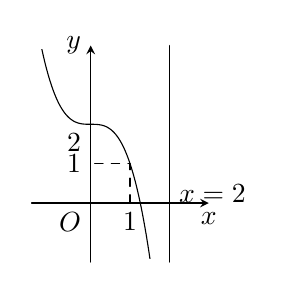
\begin{tikzpicture}[>=stealth,scale=0.5, line join=round, line cap=round]
            \def\a{-1} \def\b{0} \def\c{0} \def\d{2}
            \def\xt{-1.5} \def\xp{3} \def\yt{4} \def\yd{-1.5}
            \draw[->] (\xt,0)--(\xp,0) node [below]{$x$};
            \draw[->] (0,\yd)--(0,\yt) node [left]{$y$};
            \node at (0,0) [below left]{$O$};
            \node at (0,2) [below left]{$2$};
            \draw[dashed] (1,0)node[below]{$1$}--(1,1)--(0,1)node[left]{$1$};
            \draw (2,-1.5)--(2,0.25)node[right]{$x=2$} --(2,4);
            \clip (\xt-0.1,\yd+0.1) rectangle (\xp-0.1,\yt-0.1);
            \draw[smooth,samples=300] plot(\x,{\a*(\x)^3+\b*(\x)^2+\c*(\x)+\d});
        \end{tikzpicture}
    }
    \loigiai{
        Từ đồ thị ta suy ra đáp án đúng là $y'\leq 0, \forall x\in \mathbb{R}$.
    }
\end{ex}
\begin{ex}%[2D1Y5-1]
    \immini
    {
        Cho đồ thị của hàm số như hình vẽ bên dưới. Hỏi đồ thị là hàm số nào?
        \choice
        {\True $y=(x-1)^3$}
        {$y=x^3+1$}
        {$y=x^3-1$}
        {$y=(x+1)^3$}
    }
    {
        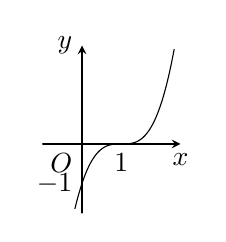
\begin{tikzpicture}[>=stealth,scale=0.5, line join=round, line cap=round]
            \def\xt{-1} \def\xp{2.5} \def\yt{2.5} \def\yd{-1.75}
            \draw[->] (\xt,0)--(\xp,0) node [below]{$x$};
            \draw[->] (0,\yd)--(0,\yt) node [left]{$y$};
            \node at (0,0) [below left]{$O$};
            \node at (0,-1) [left]{$-1$};
            \node at (1,0) [below]{$1$};
            \clip (\xt-0.1,\yd+0.1) rectangle (\xp-0.1,\yt-0.1);
            \draw[smooth,samples=300] plot(\x,{(\x-1)^3});
        \end{tikzpicture}
    }
    \loigiai{
        Dựa vào đồ thị hàm số ta có đáp án cần tìm là $y=(x-1)^3$.
    }
\end{ex}
\begin{ex}%[2D1Y5-1]
    \immini
    {
        Cho hàm số $y=ax^3+bx^2+cx+d$ có đồ thị như hình. Mệnh đề nào sau đây {\bf đúng}?
        \choice
        {$y'=0$ vô nghiệm}
        {$y'=0$ có $1$ nghiệm duy nhất}
        {$y'=0$ có $2$ nghiệm phân biệt}
        {$y'=0$ có $3$ nghiệm}
    }
    {
        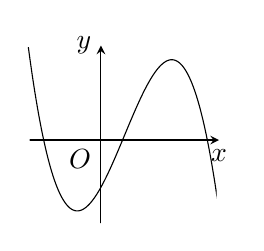
\begin{tikzpicture}[>=stealth,scale=.3, line join=round, line cap=round]
            \def\a{-1/5} \def\b{3/5} \def\c{9/5} \def\d{-2}
            \def\xt{-3} \def\xp{5} \def\yt{4} \def\yd{-3.5}
            \draw[->] (\xt,0)--(\xp,0) node [below]{$x$};
            \draw[->] (0,\yd)--(0,\yt) node [left]{$y$};
            \node at (0,0) [below left]{$O$};
            \clip (\xt-0.1,\yd+0.1) rectangle (\xp-0.1,\yt-0.1);
            \draw[smooth,samples=300] plot(\x,{\a*(\x)^3+\b*(\x)^2+\c*(\x)+\d});
        \end{tikzpicture}
    }
    \loigiai{
        Từ đồ thị hàm số, ta thấy hàm số có $2$ cực trị, do đó phương trình $y'=0$ có $2$ nghiệm phân biệt.
    }
\end{ex}
\begin{ex}
    \immini{Bảng biến thiên ở hình bên là của một trong bốn hàm số sau đây. Hỏi đó là hàm số nào?
        \choice
        {$y=-x^3-2x^2+5$}
        {\True $y=x^3-3x^2+5$}
        {$y=-x^3-3x+5$}
        {$y=x^3+3x^2+5$}}{
        
\begin{tikzpicture}
            \tkzTabInit[nocadre=false, lgt=1.2, espcl=1.6]{$x$ /0.6,$f'(x)$ /0.6,$f(x)$ /1.5}{$-\infty$,$0$,$2$,$+\infty$}
            \tkzTabLine{,+,$0$,-,$0$,+,}
            \tkzTabVar{-/ $-\infty$/, +/$5$ , -/$1$ , +/$+\infty$/}
    \end{tikzpicture}}
\end{ex}
\begin{ex}
    \immini{Bảng biến thiên ở hình bên là của một trong bốn hàm số sau đây. Hỏi đó là hàm số nào?
        \choice
        {$ y=-x^3+3x^2 $}
        {$ y=x^3-3x^2-1$}
        {$ y=x^4+2x^2+1 $}
        {\True$ y=-x^3+3x^2+1 $}}{
        
\begin{tikzpicture}
            \tkzTabInit[nocadre=false,lgt=1.2,espcl=1.6,deltacl=0.6]
            {$x$/0.6, $y'$/0.6, $y$/1.5}
            {$-\infty$,$0$,$2$,$+\infty$}
            \tkzTabLine{,-,z,+,z,-,}
            \tkzTabVar{+/$+\infty$ ,-/ $1$ ,+/$5$, -/$-\infty$}
    \end{tikzpicture}}
    \loigiai{
        Ta thấy đây là hàm số bậc ba và $\displaystyle\lim\limits_{x\rightarrow-\infty}=-\infty$ nên $a<0$.\\
        Ta có $f(0)=1$ nên hàm số cần tìm là $y=-x^3+3x^2+1$.
    }
\end{ex}
\begin{ex}
    \immini{Bảng biến thiên ở hình bên là của một trong bốn hàm số sau đây. Hỏi đó là hàm số nào?
        \haicot
        {$y=x^3-3x^2+x+3$}
        {$y=x^3-3x+4$}
        {\True $y=x^3-3x^2+3x+1$}
        {$y=x^3+3x^2+5$}}{
        
\begin{tikzpicture}
            \tkzTabInit[lgt=1,espcl=2.5]
            {$x$/0.6,$y'$/0.6,$y$/1.5}
            {$-\infty$,$1$,$+\infty$}
            \tkzTabLine{,+,$0$,+,}
            \tkzTabVar{-/$-\infty$,R,+/$+\infty$}
            \tkzTabIma[draw]{1}{3}{2}{$2$}
    \end{tikzpicture}}
\end{ex}
\begin{ex}%[2D1B5-1]
    \immini{Đường cong bên là đồ thị của một trong bốn hàm số đã cho sau đây. Hỏi đó là hàm số nào?
        \choice
        {$y=-x^3+x^2-2$}
        {\True $y=x^3+3x^2-2$}
        {$y=x^3-3x+2$}
        {$y=x^2-3x-2$}
    }{
        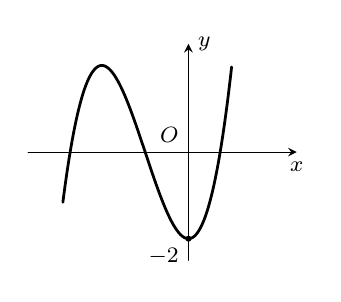
\begin{tikzpicture}[scale=0.55, font=\footnotesize,line join=round, line cap=round,>=stealth]
            \draw[->] (-3.7,0.) -- (2.5,0.) node[below]{$x$};
            \draw[->] (0,-2.5) -- (0,2.5) node[right]{$y$};
            \fill (0,0) node[above left]{$O$};
            \fill (0,-2) circle(2pt) node[below left]{$-2$};
            \draw[line width=1pt,smooth,samples=300,domain=-2.9:1] plot(\x,{(\x+2)^3-3*(\x+2)^2+2});
        \end{tikzpicture}
    }
    \loigiai{
        Dựa vào hình dáng đồ thị, ta thấy đây là đồ thị của hàm số bậc ba $y=ax^3+bx^2+cx+d$ với $a>0$ nên loại các hàm $y=x^4+x^2-2$, $y=-x^2-3x-2$. Mặt khác, đồ thị đi qua điểm $(0;-2)$ nên loại hàm $y=x^3-3x+2$.\\
        (Ngoài ra, ta có thể đánh giá dấu của các hệ số $a,~b,~c$ thông qua hoành độ $2$ điểm cực trị và hoành độ trung điểm của hai điểm cực trị. Trong đồ thị này ta còn thấy hàm số có điểm cực tiểu $x=0$ nên $c=0$)
    }
\end{ex}
\begin{ex}%
    \immini{Đường cong bên là đồ thị của một trong bốn hàm số đã cho sau đây. Hỏi đó là hàm số nào?
        \choice
        {$y=x^3+3x-2 $}
        {$ y=x^3-3x+2$}
        {\True $y=-x^3+3x+2$}
        {$y=-x^3-3x-2$}
    }{
        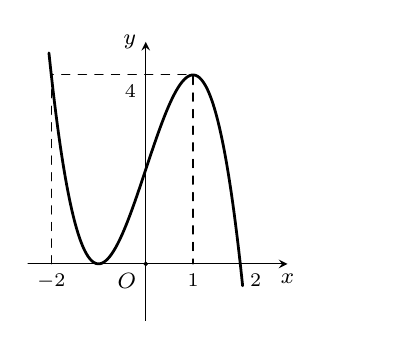
\begin{tikzpicture}[scale=0.6, font=\footnotesize, line join=round, line cap=round, >=stealth]
            \clip(-2.5,-1.2) rectangle (5,5);
            \draw[->] (-2.5,0) -- (3,0) node[below]{ $x$};
            \draw[->] (0,-1.5) -- (0,4.7) node[left]{ $y$};
            \draw[line width=1pt,smooth,samples=100,domain=-2.05:2.05] plot(\x,{-(\x)^3+3*(\x)+2});
            \draw [fill=black] (0,0) circle (1pt)node[below left]{\footnotesize $O$}(-1,1);
            \draw[dashed](-2,0)node[below]{\scriptsize $-2$}--(-2,4)--(0,4)node[below left]{\scriptsize $4$}--(1,4)--(1,0)node[below]{\scriptsize $1$};
            \draw(2,0)node[below right]{\scriptsize $2$};
    \end{tikzpicture}}
    \loigiai{
        Quan sát đồ thị, ta thấy nhánh cuối của đồ thị hướng xuống dưới nên $\lim\limits_{x\rightarrow +\infty}y=-\infty$, suy ra hệ số $a<0$. Như vậy hai hàm số 	$y=x^3+3x-2; y=x^3-3x+2$ không thỏa mãn.
        \\Mặt khác hàm số có hai điểm cực trị nên hàm số $y=-x^3-3x-2$ có $y'=-3x^2-3<0$ $\forall x\in \mathbb{R}$ không thỏa mãn.
    }
\end{ex}
\begin{ex}
    \immini{Đường cong bên là đồ thị của một trong bốn hàm số đã cho sau đây. Hỏi đó là hàm số nào?
        \choice
        {$y=x^3-3x^2-4$}
        {$y=-x^3-4$}
        {$y=-x^3+3x^2-2$}
        {\True $y=-x^3+3x^2-4$}
    }{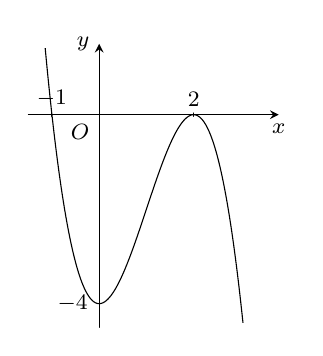
\begin{tikzpicture}[scale=0.6,>=stealth, font=\footnotesize, line join=round, line cap=round]
            \def\a{-1} \def\b{3} \def\c{0} \def\d{-4} % Hệ số
            \def\xmin{-1.5} \def\xmax{3.8}
            \def\ymin{-4.5} \def\ymax{1.5}
            %\draw[color=gray!50,dashed] (\xmin,\ymin) grid (\xmax,\ymax);
            \foreach \x in {-1,2}
            \draw[thin] (\x,1pt)--(\x,-1pt) node [above] {$\x$};
            \foreach \y in {-4}
            \draw[thin] (1pt,\y)--(-1pt,\y) node [left] {$\y$};
            \draw[->] (\xmin,0)--(\xmax,0) node [below]{$x$};
            \draw[->] (0,\ymin)--(0,\ymax) node [left]{$y$};
            \node at (0,0) [below left]{$O$};
            \clip (\xmin+0.1,\ymin+0.1) rectangle (\xmax-0.5,\ymax-0.1);
            \draw[smooth,samples=300] plot(\x,{\a*(\x)^3+\b*(\x)^2+\c*(\x)+\d});
    \end{tikzpicture}}
    \loigiai{
        \begin{itemize}
            \item Đồ thị hàm số có dạng chữ N ngược nên đây là đồ thị hàm số $y=ax^3+bx^2+cx+d$ với $a<0$. Loại phương án $y=x^3-3x^2-4$.
            \item Đồ thị hàm số giao $Oy$ tại điểm có tung độ bằng $-4$ nên $d=-4$, loại phương án $y=-x^3+3x^2-2$.
            \item Hàm số có hai điểm cực trị $x=0, x=2$ nên loại phương án $y=-x^3-4$ (vì phương án này có $y'=-3x^2$, hàm số không có điểm cực trị).
    \end{itemize}}
\end{ex}
\begin{ex}
    \immini{Đường cong bên là đồ thị của một trong bốn hàm số đã cho sau đây. Hỏi đó là hàm số nào?
        \haicot
        {$y=x^3-1$}
        {$y=(x+1)^3$}
        {\True $y=(x-1)^3$}
        {$y=x^3+1$}}
    {
        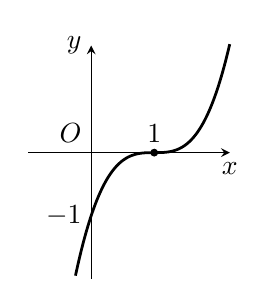
\begin{tikzpicture}[scale=0.8,>=stealth]
            \draw[->] (-1,0)--(0,0)node[above left]{$O$}--(2.2,0)node[below]{$x$};
            \draw[->] (0,-2)--(0,1.7)node[left]{$y$};
            \draw[line width=1pt,smooth,samples=100,domain=-0.25:2.2] plot(\x,{(\x-1)^3});
            \draw [fill=black] (1,0) circle (1.5pt);
            \draw (1,0)node[above]{$1$} (0,-1)node[left]{$-1$};
        \end{tikzpicture}
    }
    \loigiai{
        $(C)$ tiếp xúc với $Ox$ tại điểm uốn, suy ra $f(x)$ có nghiệm bội ba $x=1$ nên hàm số có dạng $y=a(x-1)^3$. Mà $(0;-1)\in (C)$ nên $a=1$.
    }
\end{ex}
\begin{ex}
    \immini{Cho hàm số $y = ax^3 + bx^2 + cx + d$ có đồ thị như hình vẽ bên. Khẳng định nào sau đây là đúng?
        \choice
        {$a > 0$, $b > 0$, $c > 0$, $d > 0$}
        {$a < 0$, $b < 0$, $c > 0$, $d > 0$}
        {$a > 0$, $b < 0$, $c < 0$, $d > 0$}
        {\True $a > 0$, $b < 0$, $c > 0$, $d > 0$}}
    {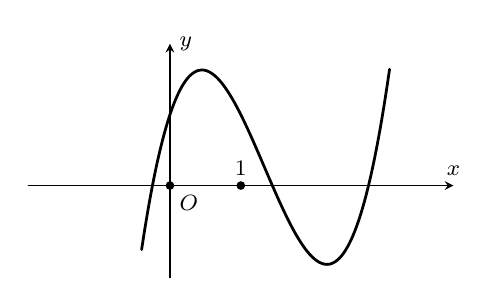
\begin{tikzpicture}[scale=0.9, font= \footnotesize, line join=round, line cap=round, >=stealth]
            \draw[->] (-2,0) -- (4,0) node[above] {$x$};
            \draw[->] (0,-1.3) -- (0,2) node[right] {$y$};
            \draw[fill=black] (1,0) circle (1.5pt);
            \draw[fill=black] (0,0) circle (1.5pt);
            \draw[line width=1pt,smooth,samples=100,domain=-0.4:3.1] plot(\x,{(\x)^3-4*(\x)^2 + 3*(\x) + 1});
            \node[below right] at (0,0) {$O$};
            \node[above] at (1,0) {$1$};
    \end{tikzpicture}}
    \loigiai{
        Nhìn vào đồ thị, ta thấy đồ thị hàm số đi từ $-\infty$ lên $+\infty$ nên $a > 0$. \\
        Giao điểm với trục tung nằm trên trục hoành, do đó $d > 0$.\\
        Hàm số có hai điểm cực trị, và hai điểm cực trị đều dương. Suy ra tổng hai điểm cực trị và tích hai điểm cực trị đều dương.\\ 	Ta có $f'(x) = 3ax^2 + 2bx + c$ nên tổng hai điểm cực trị là $\dfrac{-2b}{3a}$. Suy ra $\dfrac{-2b}{3a} > 0$, hay $b < 0$.\\ Còn tích hai điểm cực trị là $\dfrac{c}{3a}$. Suy ra $\dfrac{c}{3a} > 0$ hay $c > 0$.}
\end{ex}
\begin{ex}%[2D1B5-1]
    \immini{Cho hàm số $ y=ax^3+bx^2+cx+d $ có đồ thị như hình vẽ bên. Mệnh đề nào sau đây đúng?
        \choice
        {$ a<0 $, $ b<0 $, $ c<0 $, $ d>0 $}
        {$ a<0 $, $ b>0 $, $ c<0 $, $ d>0 $}
        {\True $ a<0 $, $ b>0 $, $ c>0 $, $ d<0 $}
        {$ a<0 $, $ b<0 $, $ c>0 $, $ d<0 $}}{
        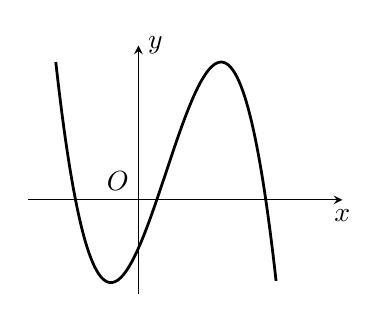
\begin{tikzpicture}[smooth,samples=300,scale=0.7,>=stealth]
            \draw[->] (-2,0)--(3.7,0) node[below]{$x$};
            \draw[->] (0,-1.7)--(0,2.8) node[right]{$y$};
            \draw (0,0) node[above left]{$O$};
            \draw[line width=1pt,domain=-1.5:2.5] plot(\x,{-(\x-0.5)^3+3*(\x-0.5)+0.5});
        \end{tikzpicture}
    }
    \loigiai{
        Dựa vào hình dáng đồ thị suy ra $ a<0 $.\\
        Dựa vào vị trí điểm cực đại và điểm cực tiểu, suy ra $ x_{\text{CT}}+x_{\text{CĐ}}>0 \Rightarrow -\dfrac{b}{a}>0\Rightarrow b>0$.\\
        Hai điểm cực trị có hoành độ trái dấu nên $ x_{\text{CT}}\cdot x_{\text{CĐ}}<0\Rightarrow \dfrac{c}{a}<0\Rightarrow c>0 $.\\
        Đồ thị hàm số cắt trục tung tại điểm có tung độ dương nên $ d>0 $.\\
        Vậy $ a<0 $, $ b>0 $, $ c>0 $ và $ d>0 $.
    }
\end{ex}
\begin{ex}%[2D1K5-1]
    \immini{Cho hàm số $y=ax^3+bx^2+cx+d$ có đồ thị như hình vẽ bên. Mệnh đề nào dưới đây đúng?
        \choice
        {$a<0$, $b>0$, $c>0$, $d>0$}
        {$a<0$, $b<0$, $c=0$, $d>0$}
        {\True $a<0$, $b>0$, $c=0$, $d>0$}
        {$a>0$, $b<0$, $c>0$, $d>0$}}{
        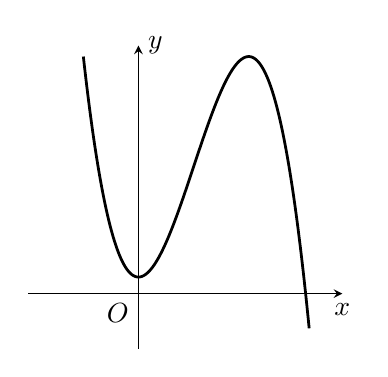
\begin{tikzpicture}[smooth,samples=300,scale=0.7,>=stealth]
            \draw[->] (-2,0)--(3.7,0) node[below]{$x$};
            \draw[->] (0,-1)--(0,4.5) node[right]{$y$};
            \draw (0,0) node[below left]{$O$};
            \draw[line width=1pt,domain=-1:3.1] plot(\x,{-(\x)^3+3*(\x)^2+0.3});
            %\draw[fill=black] (2,-1) circle(1.5pt) (2,0) circle(1pt) (0,-1) circle(1pt);
            %\draw[dashed] (2,-1.5)--(2,2.5) (2,-1)--(0,-1)node[left]{\small$-\dfrac{\Delta}{4a}$};
            %\node[right] at (2,2.4) {\small $x=-\tfrac{b}{2a}$};
            %\node[right] at (0.5,-2) {\fbox{$a>0$}};
        \end{tikzpicture}
    }
    \loigiai{
        Dựa vào đồ thị ta có thể thấy $a<0$, đồ thị cắt trục tung tại điểm có tung độ dương nên $d>0$.\\
        Hàm số có hai cực trị thỏa $\heva{&S>0\\&P=0}\Leftrightarrow\heva{&-\dfrac{b}{a}>0\\&\dfrac{c}{a}=0}\Leftrightarrow\heva{&b>0\\&c=0.}$
    }
\end{ex}
\begin{ex}
    \immini{Cho hàm số $y=ax^3+bx^2+cx+d$ có bảng biến
        thiên như hình bên. Trong các hệ số $a$, $b$, $c$ và $d$ có bao nhiêu số âm?
        \choice
        {$2$}
        {\True $1$}
        {$4$}
        {$3$}}{
        
\begin{tikzpicture}[>=stealth,scale=1]
            \tkzTabInit[lgt=1.2,espcl=2]
            {$x$ /0.6, $f’(x)$ /0.6, $f(x)$ /2}
            {$-\infty$,$-1$,$2$,$+\infty$}
            \tkzTabLine{ ,-,z,+,z,-, }
            \tkzTabVar{+/,-/$0$,+/,-/}
    \end{tikzpicture}}
    \loigiai
    {
        Từ bảng biến thiên ta thấy hàm số có $2$ điểm cực trị nên bậc của đa thức phải lớn hơn $2\Rightarrow a\ne 0$. Mà $\lim \limits_{x \to +\infty} y=-\infty\Rightarrow a<0$.\\
        Từ bảng biến thiên ta có $d=y(0)>y(-1)=0$.\\
        Ta có $y'=3ax^2+2bx+c$ có hai nghiệm là $-1$ và $2$ nên $\heva{& -\dfrac{2b}{3a}=-1+2=1>0 \\ & \dfrac{c}{3a}=(-1)\cdot 2=-2<0}\Rightarrow \heva{& b>0 \\ & c>0.}$
    }
\end{ex}
\begin{ex}%[2D1K5-1]
    \immini
    {
        Cho đồ thị hàm số bậc ba $y=ax^3+bx^2+cx+d$ như hình vẽ bên dưới. Có bao nhiêu số dương trong các số $a,b,c,d$?
        \choice
        {$1$}
        {\True $2$}
        {$3$}
        {$4$}
    }
    {
        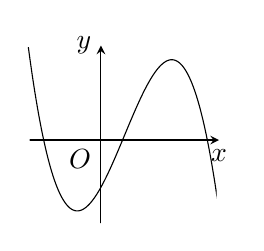
\begin{tikzpicture}[>=stealth,scale=0.3, line join=round, line cap=round]
            \def\a{-1/5} \def\b{3/5} \def\c{9/5} \def\d{-2} % Hệ số
            \def\xt{-3} \def\xp{5} \def\yt{4} \def\yd{-3.5}
            \draw[->] (\xt,0)--(\xp,0) node [below]{$x$};
            \draw[->] (0,\yd)--(0,\yt) node [left]{$y$};
            \node at (0,0) [below left]{$O$};
            \clip (\xt-0.1,\yd+0.1) rectangle (\xp-0.1,\yt-0.1);
            \draw[smooth,samples=300] plot(\x,{\a*(\x)^3+\b*(\x)^2+\c*(\x)+\d});
        \end{tikzpicture}
    }
    \loigiai{
        Từ đồ thị hàm số, ta thấy $a,d<0$.\\
        Hàm số đạt $2$ tại hai điểm $x_1<0<x_2$ và $x_2>|x_1|$, do đó\\
        $y'=a(x-x_1)(x-x_2)=ax^2-a(x_1+x_2)x+ax_1x_2$, hay $b=-a(x_1+x_2)>0$ và $c=ax_1x_2>0$.\\
        Vậy đáp án là có $2$ hệ số dương.
    }
\end{ex}
\begin{ex}%[2D1K5-1]
    \immini
    {
        Cho đồ thị hàm số bậc ba $y=ax^3+bx^2+cx+d$ như hình vẽ bên dưới. Có bao nhiêu số dương trong các số $a,b,c,d$?
        \choice
        {\True $1$}
        {$2$}
        {$3$}
        {$4$}
    }
    {
        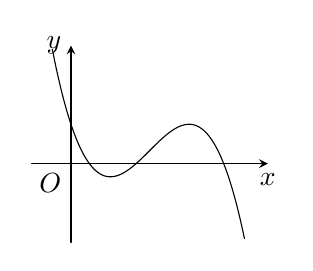
\begin{tikzpicture}[>=stealth,scale=0.5, line join=round, line cap=round]
            \def\a{-1/3} \def\b{2} \def\c{-3} \def\d{1} % Hệ số
            \def\xt{-1} \def\xp{5} \def\yt{3} \def\yd{-2}
            \draw[->] (\xt,0)--(\xp,0) node [below]{$x$};
            \draw[->] (0,\yd)--(0,\yt) node [left]{$y$};
            \node at (0,0) [below left]{$O$};
            \clip (\xt-0.1,\yd+0.1) rectangle (\xp-0.1,\yt-0.1);
            \draw[smooth,samples=300] plot(\x,{\a*(\x)^3+\b*(\x)^2+\c*(\x)+\d});
        \end{tikzpicture}
    }
    \loigiai{
        Từ đồ thị hàm số, ta có $a<0$ và $d>0$.\\
        Đồ thị hàm số đạt cực trị tại hai điểm có hoành độ đương nên ta có $S,P>0$ hay $\dfrac{-b}{a}>0$ và $\dfrac{c}{a}>0$ mà $a<0$ do đó $b>0,c<0$.
    }
\end{ex}
\begin{ex}%[2D1K5-1]
    \immini
    {
        Cho đồ thị hàm số $y=ax^3+bx^2+cx+d$ như hình vẽ. tìm mệnh đề {\bf đúng}?
        \choice
        {$a>0,b>0,c<0,d<0$}
        {$a<0,b>0,c<0,d>0$}
        {\True $a>0,b<0,c>0,d>0$}
        {$a<0,b<0,c>0,d<0$}
    }
    {
        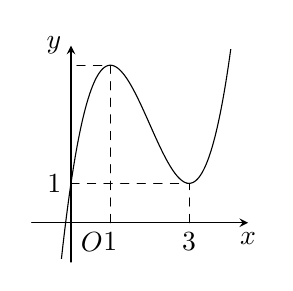
\begin{tikzpicture}[>=stealth,scale=.5, line join=round, line cap=round]
            \def\a{3/4} \def\b{-9/2} \def\c{27/4}
            \def\d{1}
            \def\xt{-1} \def\xp{4.5} \def\yt{4.5} \def\yd{-1}
            \draw[->] (\xt,0)--(\xp,0) node [below]{$x$};
            \draw[->] (0,\yd)--(0,\yt) node [left]{$y$};
            \node at (0,0) [below right]{$O$};
            \draw[dashed] (1,0)node[below]{$1$}--(1,4)--(0,4);
            \draw[dashed] (3,0)node[below]{$3$}--(3,1)--(0,1)node[left]{$1$};
            \clip (\xt-0.1,\yd+0.1) rectangle (\xp-0.1,\yt-0.1);
            \draw[smooth,samples=300] plot(\x,{\a*(\x)^3+\b*(\x)^2+\c*(\x)+\d});
        \end{tikzpicture}
    }
    \loigiai{
        Từ đồ thị ta có $a>0,d=1>0$ đo đó đáp án đúng là $a>0,b<0,c>0,d>0$.
    }
\end{ex}
\begin{ex}%[2D1K5-1]
    \immini
    {
        Cho đồ thị hàm số $y=ax^3+bx^2+cx+d$ như hình vẽ bên dưới. Tìm mệnh đề {\bf đúng}?
        \choice
        {\True $a>0,b>0,c=0,d<0$}
        {$a>0,b>0,c=0,d>0$}
        {$a>0,b>0,c>0,d>0$}
        {$a>0,b<0,c=0,d<0$}
    }
    {
        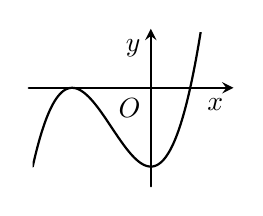
\begin{tikzpicture}[line join=round, line cap=round,>=stealth,thick, scale=0.5]
            \tikzset{label style/.style={font=\footnotesize}}
            \draw[->] (-3.1,0)--(2.1,0) node[below left] {$x$};
            \draw[->] (0,-2.5)--(0,1.5) node[below left] {$y$};
            \draw (0,0) node [below left] {$O$};
            \begin{scope}
                \clip (-3,-2.5) rectangle (2,1.4);
                \draw[samples=200,domain=-3:1.5,smooth,variable=\x] plot (\x,{0.5*((\x)^3)+1.5*((\x)^2)+0*(\x)+-2});
            \end{scope}
        \end{tikzpicture}
    }
    \loigiai{
        Từ đồ thị ta thấy hàm số có hệ số $a>0, d<0$.\\
        Hàm số đạt cực trị tại điểm có hoành độ âm và hoành độ bằng $0$ do đó $c=0$ và $b>0$.
    }
\end{ex}
\begin{ex}%[2D1K5-1]
    \immini
    {
        Cho đồ thị hàm số $y=ax^3+bx^2+cx+d \ (a,b,c,d \in \mathbb{R})$ như hình vẽ. Có bao nhiêu số dương trong các số $a,b,c,d$?
        \choice
        {\True $1$}
        {$2$}
        {$3$}
        {$4$}
    }
    {
        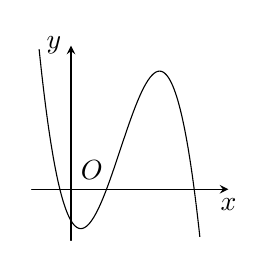
\begin{tikzpicture}[>=stealth,scale=0.5, line join=round, line cap=round]
            \def\a{-1} \def\b{6} \def\c{-9} \def\d{-1}
            \def\xt{-1} \def\xp{4} \def\yt{3.65} \def\yd{-1.3}
            \draw[->] (\xt,0)--(\xp,0) node [below]{$x$};
            \draw[->] (0,\yd)--(0,\yt) node [left]{$y$};
            \node at (0,0) [above right]{$O$};
            \clip (\xt-0.1,\yd+0.1) rectangle (\xp-0.1,\yt-0.1);
            \draw[smooth,samples=300] plot(\x,{\a*(\x+0.75)^3+\b*(\x+0.75)^2+\c*(\x+0.75)+\d+4});
        \end{tikzpicture}
    }
    \loigiai{
        Từ đồ thị hàm số ta thấy $a,d<0$.\\
        Ta có $y'=3ax^2+2bx+c$.\\
        Đồ thị hàm số có $2$ điểm cực trị có hoành độ dương nên do đó $\heva{&-\dfrac{b}{a}>0\\&\dfrac{c}{a}>0}$ do đó $b>0,c<0$.\\
        Vậy có $1$ hệ số dương.
    }
\end{ex}
\begin{ex}%[2D1K5-1]
    \immini
    {
        Cho đồ thị hàm số $y=ax^3+bx^2+cx+d \ (a,b,c,d \in \mathbb{R})$ như hình vẽ. Có bao nhiêu số dương trong các số $a,b,c,d$?
        \choice
        {\True $1$}
        {$2$}
        {$3$}
        {$4$}
    }
    {
        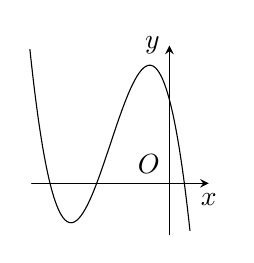
\begin{tikzpicture}[>=stealth,scale=0.5, line join=round, line cap=round]
            \def\a{-1} \def\b{6} \def\c{-9} \def\d{-1}
            \def\xt{-3.5} \def\xp{1} \def\yt{3.5} \def\yd{-1.3}
            \draw[->] (\xt,0)--(\xp,0) node [below]{$x$};
            \draw[->] (0,\yd)--(0,\yt) node [left]{$y$};
            \node at (0,0) [above left]{$O$};
            \clip (\xt-0.1,\yd+0.1) rectangle (\xp-0.1,\yt-0.1);
            \draw[smooth,samples=300] plot(\x,{\a*(\x+3.5)^3+\b*(\x+3.5)^2+\c*(\x+3.5)+\d+4});
        \end{tikzpicture}
    }
    \loigiai{
        Từ đồ thị hàm số ta thấy $a<0,d>0$.\\
        Ta có $y'=3ax^2+2bx+c$.\\
        Đồ thị hàm số có $2$ điểm cực trị có hoành độ âm nên do đó $\heva{&-\dfrac{b}{a}<0\\&\dfrac{c}{a}>0}$, do đó $b<0,c<0$.\\
        Vậy có $1$ hệ số dương.
    }
\end{ex}
\begin{ex}%[2D1K5-1]
    \immini
    {
        Cho đồ thị hàm số $y=ax^3+bx^2+cx+d \ (a,b,c,d \in \mathbb{R})$ như hình vẽ. Có bao nhiêu số dương trong các số $a,b,c,d$?
        \choice
        {\True $1$}
        {$2$}
        {$3$}
        {$4$}
    }
    {
        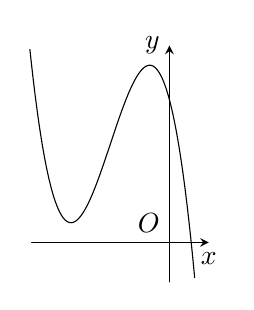
\begin{tikzpicture}[>=stealth,scale=.5, line join=round, line cap=round]
            \def\a{-1} \def\b{6} \def\c{-9} \def\d{-1}
            \def\xt{-3.5} \def\xp{1} \def\yt{5} \def\yd{-1}
            \draw[->] (\xt,0)--(\xp,0) node [below]{$x$};
            \draw[->] (0,\yd)--(0,\yt) node [left]{$y$};
            \node at (0,0) [above left]{$O$};
            \clip (\xt-0.1,\yd+0.1) rectangle (\xp-0.1,\yt-0.1);
            \draw[smooth,samples=300] plot(\x,{\a*(\x+3.5)^3+\b*(\x+3.5)^2+\c*(\x+3.5)+\d+5.5});
        \end{tikzpicture}
    }
    \loigiai{
        Từ đồ thị hàm số ta thấy $a<0,d>0$.\\
        Ta có $y'=3ax^2+2bx+c$.\\
        Đồ thị hàm số có $2$ điểm cực trị có hoành độ âm nên do đó $\heva{&-\dfrac{b}{a}<0\\&\dfrac{c}{a}>0}$ do đó $b<0,c<0$.\\
        Vậy có $1$ hệ số dương.
    }
\end{ex}
\begin{ex}%[2D1K5-1]
    \immini
    {
        Cho đồ thị hàm số $y=ax^3+bx^2+cx+d$ như hình vẽ bên dưới. Tìm mệnh đề {\bf đúng}?
        \choice
        {$a<0,b>0,c>0,d<0$}
        {$a>0,b>0,c>0,d<0$}
        {$a>0,b<0,c<0,d>0$}
        {\True $a>0,b<0,c>0,d<0$}
    }
    {
        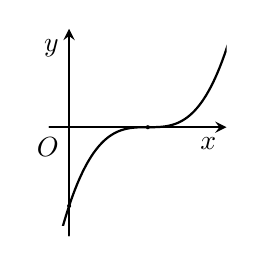
\begin{tikzpicture}[line join=round, line cap=round,>=stealth,thick, scale=0.5]
            \tikzset{label style/.style={font=\footnotesize}}
            \draw[->] (-0.5,0)--(4,0) node[below left] {$x$};
            \draw[->] (0,-2.75)--(0,2.5) node[below left] {$y$};
            \draw (0,0) node [below left] {$O$};
            \begin{scope}
                \clip (-0.5,-2.5) rectangle (4,2.5);
                \draw[samples=200,domain=-5:5,smooth,variable=\x] plot (\x,{0.25*((\x)^3)+-1.5*((\x)^2)+3*(\x)+-2});
            \end{scope}
            \fill (2,0) circle (1.5pt);
            \fill (0,-2) circle (1.5pt);
        \end{tikzpicture}
    }
    \loigiai{
        Từ đồ thị ta thấy $a>0,d<0$.\\
        Đồ thị hàm số không có cực trị và phương trình $y'=0$ có nghiệm kép $x_0>0$ đo đó $b<0,c>0$.
    }
\end{ex}
\begin{ex}%[2D1K5-1]
    \immini
    {
        Cho đồ thị hàm số $y=ax^3+bx^2+cx+d$ như hình vẽ bên dưới. Tìm mệnh đề {\bf đúng}?
        \choice
        {$ab^2>3a^2c$}
        {\True $ab^2<3a^2c$}
        {$b^2d>3acd$}
        {$-b^2d<-3acd$}
    }
    {
        \begin{tikzpicture}[>=stealth,scale=.5, line join=round, line cap=round]
            \def\a{1} \def\b{0} \def\c{1} \def\d{1} % Hệ số
            \def\xt{-1.5} \def\xp{1.5} \def\yt{3} \def\yd{-2}
            \draw[->] (\xt,0)--(\xp,0) node [below]{$x$};
            \draw[->] (0,\yd)--(0,\yt) node [left]{$y$};
            \node at (0,0) [below left]{$O$};
            \clip (\xt-0.1,\yd+0.1) rectangle (\xp-0.1,\yt-0.1);
            \draw[smooth,samples=300] plot(\x,{\a*(\x)^3+\b*(\x)^2+\c*(\x)+\d});
        \end{tikzpicture}
    }
    \loigiai{
        Ta có $y'=3ax^2+2bx+c$.\\
        Từ đồ thị hàm số ta thấy $a>0$ và phương trình $y'=0$ vô nghiệm.\\
        Hay $b^2-3ac<0\Leftrightarrow b^2<3ac\Leftrightarrow ab^2<3a^2c$.
    }
\end{ex}
\begin{ex}%[2D1K5-1]
    \immini
    {
        Cho đồ thị hàm số $y=-2x^3+bx^2+cx+d$ như hình vẽ bên dưới. Tổng $b+c+d$ bằng
        \choice
        {\True $1$}
        {$3$}
        {$5$}
        {$7$}
    }
    {
        \begin{tikzpicture}[>=stealth,scale=0.5, line join=round, line cap=round]
            \def\a{-2} \def\b{9} \def\c{-12} \def\d{4}
            \def\xt{-1} \def\xp{3} \def\yt{5.5} \def\yd{-2}
            \draw[->] (\xt,0)--(\xp,0) node [below]{$x$};
            \draw[->] (0,\yd)--(0,\yt) node [left]{$y$};
            \node at (0,0) [below left]{$O$};
            \node at (2,0) [above]{$2$};
            \node at (0,4) [right]{$4$};
            \clip (\xt-0.1,\yd+0.1) rectangle (\xp-0.1,\yt-0.1);
            \draw[smooth,samples=300] plot(\x,{\a*(\x)^3+\b*(\x)^2+\c*(\x)+\d});
            \draw[dashed] (1,0)node[above]{$1$}--(1,-1);
            \fill (0,4)circle (1.5pt);
            \fill (2,0)circle (1.5pt);
        \end{tikzpicture}
    }
    \loigiai{
        Ta thấy đồ thị hàm số cắt trục $Oy$ tại điểm có tung độ bằng $4$ nên $d=4$. Do đó hàm số có dạng $y=-2x^3+bx^2+cx+4$.\\
        Đồ thị hàm số đi qua điểm $(2,0)$ nên ta có $4b+2c=12$ (1).\\
        Hàm số đạt cực trị tại $2$ điểm $x=1$ và $x=2$, do đó $x=1,x=2$ là nghiệm của phương trình $y'=0$ (với $y'=-6x^2+2bx+c$).\\
        Do đó ta có hệ $\heva{&2b+c=6\\&4b+c=24}$ (2).\\
        Từ (1) và (2), ta suy ra $b=9;c=-12$.\\
        Vậy $b+c+d=1$.
    }
\end{ex}
\begin{ex}%[2D1K5-1]
    \immini
    {
        Cho đồ thị hàm số $y=ax^3-3x^2+cx+d$ như hình vẽ bên dưới. Tổng $a+c+d$ bằng
        \choice
        {$2$}
        {$-3$}
        {$0$}
        {$3$}
    }
    {
        \begin{tikzpicture}[>=stealth,scale=.5, line join=round, line cap=round]
            \def\a{1} \def\b{-3} \def\c{0} \def\d{2}
            \def\xt{-1.25} \def\xp{3} \def\yt{3} \def\yd{-2.5}
            \draw[->] (\xt,0)--(\xp,0) node [below]{$x$};
            \draw[->] (0,\yd)--(0,\yt) node [left]{$y$};
            \node at (0,0) [below left]{$O$};
            \node at (0,2) [above left]{$2$};
            \node at (1,0) [below left]{$1$};
            \clip (\xt-0.1,\yd+0.1) rectangle (\xp-0.1,\yt-0.1);
            \draw[smooth,samples=300] plot(\x,{\a*(\x)^3+\b*(\x)^2+\c*(\x)+\d});
            \fill (0,2)circle (1.5pt);
            \draw[dashed] (2,0)node[above]{$2$}--(2,-2)--(0,-2)node[left]{$-2$};
        \end{tikzpicture}
    }
    \loigiai{
        Ta thấy đồ thị hàm số có một điểm cực trị là $(0;2)$ nên ta có $c=0;d=2$.\\
        Vậy hàm số cần tìm có dạng $y=ax^3-3x^2+2$.\\
        Vì đồ thị hàm số đi qua điểm có tọa độ $(2;-2)$ nên ta có $-2=8a-12+2\Leftrightarrow a=1$.\\
        Vậy $a+c+d=3$.
    }
\end{ex}
\begin{ex}%[2D1Y5-1]
    \immini{
        Đường cong trong hình vẽ là đồ thị của hàm số nào dưới đây?
        \choice
        {$y = \dfrac{2x - 1}{x - 1}$}
        {\True $y = \dfrac{x + 1}{x - 1}$}
        {$y = x^4 + x^2 +1$}
        {$y = x^3 - 3x - 1$}
    }{
        \begin{tikzpicture}[scale=0.5, font=\footnotesize, line join=round, line cap=round, >=stealth]
            \clip(-3,-2) rectangle (5.1,4.1);
            \draw[->] (-3,0) -- (5,0);\draw (4.9,0) node[below] {\small $x$};
            \draw[->] (0,-2) -- (0,4);\draw (0,3.9) node[right] {\small $y$};
            \draw[fill=black] (0,0) node[below right]{$O$} circle (1pt);
            \draw (1,0) node[below right]{$1$};
            \draw (0,1) node[above left]{$1$};
            \draw plot[domain=-3:0.5, samples=100] (\x, {(1 + \x)/(\x - 1)});
            \draw plot[domain= 1.5:5, samples=100] (\x, {(1 + \x)/(\x - 1)});
            \draw [-,dashed] (-3,1)--(5,1); %TCN
            \draw [-,dashed] (1,-2)--(1,4); %TCĐ
            \draw[fill=black] (0,0) circle(1pt);
        \end{tikzpicture}
    }
    \loigiai{
        Đường cong có đường tiệm cận đứng $ x=1 $ và tiệm cận ngang $ y=1 $ nên nó không thể là đồ thị của hàm đa thức. Ta xét các trường hợp sau:
        \begin{enumerate}
            \item Xét $ y=\dfrac{2x-1}{x-1} $, có\\
            $ \lim\limits_{x\to -\infty}\dfrac{2x-1}{x-1}=\lim\limits_{x\to +\infty}\dfrac{2x-1}{x-1}=2\Rightarrow y=2 $ là tiệm cận ngang của đồ thị hàm số. Do đó đường cong trên không thể là đồ thị của hàm số $ y=\dfrac{2x-1}{x-1} $.
            \item Xét $ y=\dfrac{x+1}{x-1} $, có\\
            $ \lim\limits_{x\to -\infty}\dfrac{x+1}{x-1}=\lim\limits_{x\to +\infty}\dfrac{x+1}{x-1}=1\Rightarrow y=1 $ là tiệm cận ngang của đồ thị hàm số.\\
            $ \lim\limits_{x\to 1^{+}}\dfrac{x+1}{x-1}=+\infty$ và $\lim\limits_{x\to 1^{-}}\dfrac{x+1}{x-1}=-\infty \Rightarrow x=1 $ là tiệm cận đứng của đồ thị hàm số.\\
            Do đó đường cong trên là đồ thị của hàm số $ y=\dfrac{x+1}{x-1} $.
        \end{enumerate}
    }
\end{ex}
\begin{ex}%[2D1Y5-1]
    \immini{Đồ thị hình bên là đồ thị của hàm số nào dưới đây?
        \choice
        { $ y = \dfrac{3 - 2x}{x+1}$}
        {$y = \dfrac{1 - 2x}{x -1}$}
        {$ y = \dfrac{1 - 2x}{1 - x}$}
        {\True $y = \dfrac{1 - 2x}{x+1}$}}
    {
        \begin{tikzpicture}[line cap=round,line join=round,>=stealth ,scale=0.4]
            \draw[->,color=black] (-6,0) -- (4,0);
            \draw[->,color=black] (0,-7) -- (0,3);
            \foreach \x in {-5,-4,-3,-2,-1,1,2,3}
            \draw[shift={(\x,0)},color=black] (0pt,2pt) -- (0pt,-2pt);
            \foreach \y in {-6,-5,-4,-3,-2,-1,1,2}
            \draw[shift={(0,\y)},color=black] (2pt,0pt) -- (-2pt,0pt);
            %\draw[color=black] (0,0) node[below left] {$O$};
            \draw[color=black] (4,0) node[above] {$x$};
            \draw[color=black] (0,3) node[right] {$y$};
            %\draw[color=black] (0.5,0) node[below right] {$\frac{1}{2^$$$$$$$\%$$$$$$$^;
            \clip(-6,-7) rectangle (4,3);
            \draw[smooth,samples=100,domain=-6:-1.01] plot(\x,{((-2*\x)+1)/((\x)+1.0)});
            \draw [dashed](-6,-2) -- (4,0.-2);
            \draw[smooth,samples=100,domain=-0.99:4] plot(\x,{((-2*\x)+1)/((\x)+1.0)});
            \draw [dashed](-1,-7) -- (-1,4);
            \node[above] at (1,0){$1$};
            \node[below left] at (-1,0){$-1$};
    \end{tikzpicture}	}
    \loigiai{
        Đồ thị đã cho có tiệm cận đứng $x = -1$ và cắt $Oy$ tại điểm $(0; 1)$ nên đây là đồ thị hàm số $ y = \dfrac{1 - 2x}{x+1}$.}
\end{ex}
\begin{ex}%[2D1Y5-1]
    \immini{
        Đường cong trong hình bên là đồ thị của hàm số nào dưới đây?
        \choice
        {\True $y=\dfrac{x-1}{x+1}$}
        {$y=x^4-2x^2-1$}
        {$y=x^3-3x^2+2$}
        {$y=\dfrac{x+1}{x-1}$}
    }{
        \begin{tikzpicture}[>=stealth, scale=.3]
            \draw[->,line width = 0.6pt] (-7,0)--(0,0) node[shift={(-0.25,-0.25)}]{$O$}--(5.3,0) node[below]{$x$};
            \draw[->,line width = 0.6pt] (0,-5)--(0,0)--(0,7) node[right]{$y$};
            \draw[fill=black] (0,0) circle (1pt);
            \draw[fill=black] (-1,0) node[shift={(-0.35,-0.3)}]{$-1$} circle (1pt);
            \draw[fill=black] (0,1) node[shift={(-0.17,0.25)}]{$1$} circle (1pt);
            \draw plot[line width = 0.8pt, domain=-7:-1.335, samples=150] (\x,{(\x-1)/(\x+1)});
            \draw plot[line width = 0.8pt, domain=-0.665:5, samples=150] (\x,{(\x-1)/(\x+1)});
            \draw [dashed,-] (-1,-5)--(-1,7);
            \draw [dashed,-] (-7,1)--(5.2,1);
        \end{tikzpicture}
    }
    \loigiai{
        \begin{itemize}
            \item Đây là dạng của đồ thị của hàm phân thức $y=\dfrac{ax+b}{cx+d}$ nên hai hàm đa thức $y=x^4-2x^2-1$ và $y=x^3-3x^2+2$ bị loại.
            \item Nhận thấy đồ thị có đường tiệm cận đứng $x=-1$ nên hàm số $y=\dfrac{x+1}{x-1}$ bị loại.\\
            Hàm số $y=\dfrac{x-1}{x+1}$ có đồ thị như đường cong của đề cho.
        \end{itemize}
    }
\end{ex}
\begin{ex}%[2D1Y5-1]
    \immini{Đồ thị hình vẽ là đồ thị của hàm số nào dưới đây?
        \choice
        {$y=\dfrac{2x-1}{x-1}$}
        {\True $y=\dfrac{x+1}{x-1}$}
        {$y=x^4+x^2+1$}
        {$y=x^3-3x-1$}
    }{\begin{tikzpicture}[scale=0.6,xscale=0.6,yscale=0.8,>=stealth, font=\footnotesize, line join=round, line cap=round]
            \def\a{1} \def\b{1} \def\c{1} \def\d{-1} % Hệ số
            \def\xmin{-6} \def\xmax{4}
            \def\ymin{-4} \def\ymax{4}
            % 	 	\draw[color=gray!50,dashed] (\xmin,\ymin) grid (\xmax,\ymax);
            \draw[->] (\xmin,0)--(\xmax,0) node [below]{$x$};
            \draw[->] (0,\ymin)--(0,\ymax) node [left]{$y$};
            \node at (0,0) [above left]{$O$};
            \clip (\xmin+0.1,\ymin+0.1) rectangle (\xmax-0.1,\ymax-0.1);
            \draw[smooth,samples=300,domain=\xmin:(-\d/\c-0.1)] plot(\x,{(\a*(\x)+\b)/(\c*(\x)+\d)});
            \draw[smooth,samples=300,domain=(-\d/\c+0.1:\xmax)] plot(\x,{(\a*(\x)+\b)/(\c*(\x)+\d)});
            \draw[dashed] (-\d/\c,\ymin)--(-\d/\c,\ymax);
            \draw[dashed] (\xmin,\a/\c)--(\xmax,\a/\c);
            \draw[fill=black](1,0)node[below right]{$1$}circle(1pt)
            (0,1)node[below right]{$1$}circle(1pt)
            (-1,0)node[below left]{$-1$}circle(1pt)
            (0,-1)node[below left]{$-1$}circle(1pt)
            ;
    \end{tikzpicture}}
    \loigiai{
        Dựa vào đồ thị ta có $y=\dfrac{x+1}{x-1}$.
    }
\end{ex}
\begin{ex}%[2D1Y5-1]
    \immini{Đường cong ở hình bên là đồ thị của hàm số $y=\dfrac{a x+b}{c x+d}$. Mệnh đề nào dưới đây đúng?
        \choice
        {$y'<0$, $\forall x\ne2$}
        {$y'<0$, $\forall x\ne-1$}
        {$y'>0$, $\forall x\ne 2$}
        {\True $y'>0$, $\forall x\ne- 1$}}{\begin{tikzpicture}[scale=0.6,xscale=0.6,yscale=0.6,>=stealth, font=\footnotesize, line join=round, line cap=round]
            \def\a{2} \def\b{1} \def\c{1} \def\d{1} % Hệ số
            \def\xmin{-6} \def\xmax{4}
            \def\ymin{-4} \def\ymax{4}
            % 	 	\draw[color=gray!50,dashed] (\xmin,\ymin) grid (\xmax,\ymax);
            \draw[->] (\xmin,0)--(\xmax,0) node [below]{$x$};
            \draw[->] (0,\ymin)--(0,\ymax) node [left]{$y$};
            \node at (0,0) [below right]{$O$};
            \clip (\xmin+0.1,\ymin+0.1) rectangle (\xmax-0.1,\ymax-0.1);
            \draw[smooth,samples=300,domain=\xmin:(-\d/\c-0.1)] plot(\x,{(\a*(\x)+\b)/(\c*(\x)+\d)});
            \draw[smooth,samples=300,domain=(-\d/\c+0.1:\xmax)] plot(\x,{(\a*(\x)+\b)/(\c*(\x)+\d)});
            \draw[dashed] (-\d/\c,\ymin)--(-\d/\c,\ymax);
            \draw[dashed] (\xmin,\a/\c)--(\xmax,\a/\c);
            \draw[fill=black](-1,0)node[below left]{$-1$}circle(1pt)
            (0,2)node[above right]{$2$}circle(1pt)
            ;
    \end{tikzpicture}}
    \loigiai{
        Dựa vào đồ thị ta có 	$y'>0$, $\forall x\ne- 1$.
    }
\end{ex}
\begin{ex}%[2D1Y5-1]
    \immini
    {
        Bảng biến thiên sau là của hàm số nào?
        \choice
        {$y=\dfrac{2x-1}{x+3}$}
        {$y=\dfrac{4x-6}{x-2}$}
        {$y=\dfrac{3-x}{2-x}$}
        {\True $y=\dfrac{x+5}{x-2}$}
    }
    {
        \begin{tikzpicture}
            \tikzset{double style/.append style={double distance=1.5pt}}
            \tkzTabInit[nocadre=false,lgt=1.5,espcl=3,deltacl=0.6]
            {$x$ /0.75,$f'(x)$ /0.75,$f(x)$ /2.25}
            {$-\infty$,$2$,$+\infty$}
            \tkzTabLine{,-,d,-,}
            \tkzTabVar{+/$1$,-D+/$-\infty$/$+\infty$,-/$1$}
        \end{tikzpicture}
    }
    \loigiai{
        + Vì $x=2$ là tiệm cận đứng của hàm số nên chọn mẫu $x-2\Rightarrow$ loại ý A\\
        + Tiệm cận ngang là $y=1$ nên loại ý B\\
        + $y=\dfrac{3-x}{2-x}=\dfrac{x-3}{x-2};y'=\dfrac{1}{(x-2)^2}>0$ là hàm số đồng biến trên khoảng K $\Rightarrow$ loại C\\
        + $y=\dfrac{x+5}{x-2};y'=\dfrac{-7}{x-2}<0$ là hàm số nghịch biến trên khoảng K và có tiệm cận đứng $x=2$,tiệm cân ngang $y=1$.}
\end{ex}
\begin{ex}%[2D1K5-1]
    \immini
    {
        Cho hàm số phù hợp với bảng biến thiên. Hỏi đó là hàm số nào?
        \choice
        {$y=\dfrac{-x+2}{x-1}$}
        {\True $y=\dfrac{x+2}{x-1}$}
        {$y=\dfrac{x+2}{x+1}$}
        {$y=\dfrac{x-3}{x-1}$}
    }
    {
        \begin{tikzpicture}
            \tkzTabInit[nocadre=false,lgt=1.2,espcl=2.5,deltacl=0.6]
            {$x$ /0.6,$y'$ /0.6,$y$ /2}
            {$-\infty$,$1$,$+\infty$}
            \tkzTabLine{,-,d,-,}
            \tkzTabVar{+/$1$,-D+/$-\infty$/$+\infty$,-/$1$}
        \end{tikzpicture}
    }
    \loigiai{
        Hàm số có dạng $y=\dfrac{ax+b}{cx+d}$.
        \begin{itemize}
            \item Tiệm cận đứng $x=1 \Rightarrow -\dfrac{d}{c}=1$.
            \item Tiệm cận ngang $y=1 \Rightarrow \dfrac{a}{c}=1$.
            \item Hàm số nghịch biến nên $ad-bc<0$
        \end{itemize}
        Ta chọn $y=\dfrac{x+2}{x-1}$.
    }
\end{ex}
\begin{ex}%[2D1K5-1]
    \immini
    {
        Cho hàm số phù hợp với bảng biến thiên. Hỏi đó là hàm số nào?
        \choice
        {$y=\dfrac{2x+1}{x-2}$}
        {$y=\dfrac{x-1}{2x+2}$}
        {\True $y=\dfrac{x+1}{x-2}$}
        {$y=\dfrac{x+3}{2+x}$}
    }
    {
        \begin{tikzpicture}
            \tkzTabInit[nocadre=false,lgt=1.2,espcl=2.5,deltacl=0.6]
            {$x$ /0.6,$y'$ /0.6,$y$ /2}
            {$-\infty$,$2$,$+\infty$}
            \tkzTabLine{,-,d,-,}
            \tkzTabVar{+/$1$,-D+/$-\infty$/$+\infty$,-/$1$}
        \end{tikzpicture}
    }
    \loigiai{
        Hàm số có dạng $y=\dfrac{ax+b}{cx+d}$.
        \begin{itemize}
            \item Tiệm cận đứng $x=2 \Rightarrow -\dfrac{d}{c}=2$.
            \item Tiệm cận ngang $y=1 \Rightarrow \dfrac{a}{c}=1$.
            \item Hàm số nghịch biến nên $ad-bc<0$
        \end{itemize}
        Ta chọn $y=\dfrac{x+1}{x-2}$.
    }
\end{ex}
\begin{ex}%[2D1K5-1]
    \immini
    {
        Cho hàm số phù hợp với bảng biến thiên. Hỏi đó là hàm số nào?
        \choice
        {$y=\dfrac{x+1}{2x-1}$}
        {\True $y=\dfrac{2x-1}{x+1}$}
        {$y=\dfrac{2x+3}{x+1}$}
        {$y=\dfrac{2x-1}{x-1}$}
    }
    {
        \begin{tikzpicture}
            \tkzTabInit[nocadre=false,lgt=1.2,espcl=2.5,deltacl=0.6]
            {$x$ /0.6,$y'$ /0.6,$y$ /2}
            {$-\infty$,$-1$,$+\infty$}
            \tkzTabLine{,+,d,+,}
            \tkzTabVar{-/$2$,+D-/$+\infty$/$-\infty$,+/$2$}
        \end{tikzpicture}
    }
    \loigiai{
        Hàm số có dạng $y=\dfrac{ax+b}{cx+d}$.
        \begin{itemize}
            \item Tiệm cận đứng $x=-1 \Rightarrow -\dfrac{d}{c}=-1$.
            \item Tiệm cận ngang $y=2 \Rightarrow \dfrac{a}{c}=2$.
            \item Hàm số đồng biến nên $ad-bc>0$
        \end{itemize}
        Ta chọn $y=\dfrac{2x-1}{x+1}$.
    }
\end{ex}
\begin{ex}%[2D1K5-1]
    \immini
    {
        Cho hàm số phù hợp với bảng biến thiên. Hỏi đó là hàm số nào?
        \choice
        {\True $y=\dfrac{x+1}{2x-1}$}
        {$y=\dfrac{2x-1}{x+1}$}
        {$y=\dfrac{2x+3}{x+1}$}
        {$y=\dfrac{2x-1}{x-1}$}
    }
    {
        \begin{tikzpicture}
            \tkzTabInit[nocadre=false,lgt=1.2,espcl=2.5,deltacl=0.6]
            {$x$ /0.6,$y'$ /0.6,$y$ /2}
            {$-\infty$,$0{,}5$,$+\infty$}
            \tkzTabLine{,+,d,+,}
            \tkzTabVar{-/$0{,}5$,+D-/$+\infty$/$-\infty$,+/$0{,}5$}
        \end{tikzpicture}
    }
    \loigiai{
        Hàm số có dạng $y=\dfrac{ax+b}{cx+d}$.
        \begin{itemize}
            \item Tiệm cận đứng $x=0{,}5 \Rightarrow -\dfrac{d}{c}=0{,}5$.
            \item Tiệm cận ngang $y=0{,}5 \Rightarrow \dfrac{a}{c}=0{,}5$.
            \item Hàm số đồng biến nên $ad-bc>0$
        \end{itemize}
        Ta chọn $y=\dfrac{x+1}{2x-1}$.
    }
\end{ex}
\begin{ex}%[2D1K5-1]
    \immini{Cho hàm số $f(x)=\dfrac{ax-2}{bx+c}$ với có bảng biến thiên như hình vẽ bên. Giá trị $a+b+c$ thuộc khoảng nào dưới đây?
        \choice
        {\True $\left(-1;1\right)$}
        {$\left(-2;-1\right)$}
        {$\left(2;3\right)$}
        {$\left(1;+\infty\right)$}}
    {\begin{tikzpicture}[scale=0.7]
            \foreach \gt[count=\i from 0] in {-\infty,-3,+\infty}\path (4*\i,0) node{$\gt$};
            \foreach \gt[count=\i from 0] in {+,+} \path (4*\i+2,-1) node{$\gt$};
            \foreach \x/\y/\gt in {-1.5/0/x,-1.5/-1/f'(x),-1.5/-2.5/f(x), 0/-3/2, 3/-2/+\infty, 5/-3/-\infty,8/-2/2}\path (\x,\y) node(\x){$\gt$};
            \draw (-2,-.5)--(8.5,-.5) (-2,-1.5)--(8.5,-1.5) (-.5,.5)--(-.5,-3.5) (4,-0.6)--(4,-3.5) (4.2,-0.6)--(4.2,-3.5);
            \foreach \x/\y in {0/3,5/8}\draw[-stealth] (\x)--(\y);
        \end{tikzpicture}
    }
    \loigiai{
        Dựa vào bảng biến thiên ta có:
        \begin{itemize}
            \item $\lim\limits_{x\to\pm\infty}f(x)=2\Rightarrow y=2$ là tiệm cận ngang của đồ thị hàm số $\Rightarrow\dfrac{a}{b}=2\Rightarrow a=2b$.
            \item $\lim\limits_{x\to{3^+}}f(x)=-\infty\Rightarrow x=3$ là tiệm cận đứng của đồ thị hàm số $\Rightarrow\dfrac{-c}{b}=3\Rightarrow c=-3b$.
            \item Hàm số đồng biến trên các khoảng $\left(-\infty ;3\right)$ và $\left(3;+\infty\right)$ nên suy ra $f'(x) > 0\Rightarrow ac+2b > 0$
            $$\Leftrightarrow-6b^2+2b > 0\Leftrightarrow 0 < b <\dfrac{1}{3}\Rightarrow \heva{&0<a<\dfrac{2}{3}\\&-1<c<0}\Rightarrow-1 < a+b+c < 1.$$
        \end{itemize}
    }
\end{ex}
\begin{ex}%[2D1K5-1]
    \immini
    {
        Cho hàm số phù hợp với bảng biến thiên. Hỏi đó là hàm số nào?
        \choice
        {\True $y=\dfrac{x+1}{2x-1}$}
        {$y=\dfrac{2x-1}{x+1}$}
        {$y=\dfrac{2x+3}{x+1}$}
        {$y=\dfrac{2x-1}{x-1}$}
    }
    {
        \begin{tikzpicture}
            \tkzTabInit[nocadre=false,lgt=1.2,espcl=2.5,deltacl=0.6]
            {$x$ /0.6,$y'$ /0.6,$y$ /2}
            {$-\infty$,$0{,}5$,$+\infty$}
            \tkzTabLine{,+,d,+,}
            \tkzTabVar{-/$0{,}5$,+D-/$+\infty$/$-\infty$,+/$0{,}5$}
        \end{tikzpicture}
    }
    \loigiai{
        Hàm số có dạng $y=\dfrac{ax+b}{cx+d}$.
        \begin{itemize}
            \item Tiệm cận đứng $x=0{,}5 \Rightarrow -\dfrac{d}{c}=0{,}5$.
            \item Tiệm cận ngang $y=0{,}5 \Rightarrow \dfrac{a}{c}=0{,}5$.
            \item Hàm số đồng biến nên $ad-bc>0$
        \end{itemize}
        Ta chọn $y=\dfrac{x+1}{2x-1}$.
    }
\end{ex}
\begin{ex}%[2D1B5-1]
    \immini{Hàm số nào trong bốn hàm số dưới đây có bảng biến thiên như hình bên?
        \choice
        {$ y=\dfrac{2x-1}{x+3} $}
        {$ y=\dfrac{4x-6}{x-2} $}
        {$ y=\dfrac{3-x}{2-x}$}
        {\True $ y=\dfrac{x+5}{x-2} $}}
    {\begin{tikzpicture}
            \tikzset{double style/.append style = {draw=\tkzTabDefaultWritingColor,double=\tkzTabDefaultBackgroundColor,double distance=2pt}}
            \tkzTabInit[nocadre=false,lgt=1,espcl=2.5,deltacl=0.6]
            {$x$/0.6,$y'$/0.6,$y$/1.5}
            {$-\infty$,$2$,$+\infty$}
            \tkzTabLine{,-,d,-,}
            \tkzTabVar{+/$1$,-D+/$-\infty$/$+\infty$,-/$1$}
        \end{tikzpicture}
    }
    \loigiai{Xét hàm số $ y=\dfrac{x+5}{x-2} $ có $$\heva{&y'=\dfrac{-7}{(x-2)^2}<0, \forall x \in \mathbb{R} \setminus \{2\} \\ & \lim\limits_{x \to \pm \infty} y=1.} $$
    }
\end{ex}
\begin{ex}%[2D1B5-1]
    \immini{Hàm số nào trong bốn hàm số dưới đây có bảng biến thiên như hình bên?
        \choice
        {$y=\dfrac{x-1}{x-3}$}
        {$y=\dfrac{x-1}{-x-3}$}
        {\True $y=\dfrac{x+5}{-x+3}$}
        {$y=\dfrac{1}{x-3}$}
    }{
        \begin{tikzpicture}
            \tikzset{double style/.append style = {draw=\tkzTabDefaultWritingColor,double=\tkzTabDefaultBackgroundColor,double distance=2pt}}
            \tkzTabInit[lgt=1,espcl=2.6]
            {$x$/0.6,$y'$/0.6,$y$/1.5}{$-\infty$,$3$,$+\infty$}
            \tkzTabLine{,+,d,+,}
            \tkzTabVar{-/$-1$,+D-/$+\infty$/$-\infty$,+/$-1$}
        \end{tikzpicture}
    }
    \loigiai{Dựa vào bảng biến thiên, ta suy ra
        \begin{itemize}
            \item Hàm số nghịch biến trên từng khoảng xác định.
            \item Đồ thị hàm số nhận đường thẳng $x=2$ và đường thẳng $y=1$ làm tiệm cận đứng và tiệm cận ngang.
        \end{itemize}
        Vậy ta nhận hàm số $y=\dfrac{x+5}{x-2}$.}
\end{ex}
\begin{ex}
    \immini
    {Đường cong trong hình vẽ bên là đồ thị của một trong bốn hàm số sau. Hỏi đó là hàm số nào?
        \choice
        {\True $y=\dfrac{2x-1}{x+1}$}
        {$y=\dfrac{1-2x}{x+1}$}
        {$y=\dfrac{2x+1}{x-1}$}
        {$y=\dfrac{2x+1}{x+1}$}
    }
    {
        \begin{tikzpicture}[smooth,samples=300,scale=0.45,>=stealth]
            \draw[->] (-5,0)--(3,0) node[below]{$x$};
            \draw[->] (0,-2.5)--(0,4.5) node[right]{$y$};
            \draw (0,0) node[above left]{$O$};
            \draw[line width=1pt,domain=-0.3:3] plot(\x,{(2*\x-1)/(\x+1)});
            \draw[line width=1pt,domain=-5:-2.2] plot(\x,{(2*\x-1)/(\x+1)});
            \draw[fill=black] (0,2) circle(1.5pt) (0,-1) circle(1.5pt) (-1,0) circle(1.5pt);
            \draw (-5,2)--(3,2) (-1,-2.5)--(-1,4.5);
            \draw (0,-1) node[right]{$-1$};
            \draw (-1,0) node[below left]{$-1$};
            \draw (0,2) node[above right]{$2$};
        \end{tikzpicture}
    }
    \loigiai
    {
        Đồ thị hàm số có tiệm cận đứng là $x=-1$ nên loại đáp án $ y=\dfrac{2x+1}{x-1}$.\\
        Đồ thị hàm số đi qua điểm $A(0;-1)$ nên loại đáp án $y=\dfrac{1-2x}{x+1}$ và $ y=\dfrac{2x+1}{x+1}$.
    }
\end{ex}
\begin{ex}
    \immini{Đường cong trong hình vẽ bên là đồ thị của một trong bốn hàm số sau. Hỏi đó là hàm số nào?
        \choice
        {$y=\dfrac{x-1}{x-2}$}
        {$y=x+2$}
        {$y=x^4-3x^2+1$}
        {\True $y=\dfrac{2x+1}{x-1}$}
    }{\begin{tikzpicture}[scale=0.7, line join=round, line cap=round,font=\footnotesize,>=stealth,x=0.7cm,y=0.7cm]
            \draw[fill,->] (-5,0)--(0,0) node[below left]{$O$}circle(0.05)--(6,0) node [below] {$x$};
            \draw[->] (0,-4)--(0,6) node [left] {$y$};
            \draw[black,domain=1.75:6, samples=100]plot(\x,{(2*(\x)+1)/((\x)-1)});
            \draw[black,domain=-4.9:0.5, samples=100]plot(\x,{(2*(\x)+1)/((\x)-1)});
            \draw[black,domain=-5:6, samples=100]plot(\x,{2});
            \draw[black,domain=-4:6, samples=100, variable=\t]plot(1,\t);
            \foreach \x in {1}
            \draw (\x,0.05)--(\x,-0.05) node [below right] {\x};
            \foreach \y in {2}
            \draw (0.05,\y)--(-0.05,\y) node [below left] {\y};
    \end{tikzpicture}}
    \loigiai{
        Đồ thị hàm số như hình vẽ nhận đường thẳng $x=1$ là tiệm cận đứng.\\
        Do đó, hàm số cần tìm là $y=\dfrac{2x+1}{x-1}$.
    }
\end{ex}
\begin{ex}
    \immini{Đường cong trong hình vẽ bên là đồ thị của một trong bốn hàm số sau. Hỏi đó là đồ thị của hàm số nào?
        \haicot
        {$y=\dfrac{x-2}{x+1}$}
        {$y=\dfrac{x+2}{x-2}$}
        {\True $y=\dfrac{x-2}{x-1}$}
        {$y=\dfrac{x+2}{x-1}$}
    }
    {
        \begin{tikzpicture}[>=stealth,x=1cm,y=1cm,scale=0.6]
            \draw[->] (-3,0)--(0,0) node[below left]{$O$}--(5,0) node[above]{$x$};
            \draw[->] (0,-3) --(0,5) node[left]{$y$};
            \foreach \x in {1,2}{\draw[-] (\x,-0.1)--(\x,0.1);}
            \foreach \y in {1,2}{\draw[-] (-0.1,\y)--(0.1,\y);}
            \draw [domain=-3:0.75, samples=100] plot (\x, {(\x-2)/(\x-1)});
            \draw [domain=1.25:5, samples=100] plot (\x, {(\x-2)/(\x-1)});
            \draw [dashed](-3,1)--(5,1) (1,-3)--(1,5);
            \draw (0,1) node[below left]{$1$};
            \draw (0,2) node[above left]{$2$};
            \draw (1,0) node[below left]{$1$};
            \draw (2,0) node[below right]{$2$};
        \end{tikzpicture}
    }
    \loigiai{
        Từ đồ thị ta thấy
        \begin{itemize}
            \item Tiệm cận ngang là $y=1$, tiệm cận đứng là $x=1$ nên các hàm số $y=\dfrac{x+2}{x-2}$, $y=\dfrac{x-2}{x+1}$ không thỏa mãn.
            \item Giao điểm của đồ thị với trục tung là $(0;2)$ nên hàm số $y=\dfrac{x+2}{x-1}$ không thỏa mãn, hàm số $y=\dfrac{x-2}{x-1}$ thỏa mãn.
        \end{itemize}
    }
\end{ex}
\begin{ex}
    \immini
    {Cho hàm số $y=\dfrac{ax-b}{x+c}$ ($a,b,c\in \mathbb{R}$) có đồ thị như hình vẽ bên. Giá trị của biểu thức $2a+b-3c$ bằng
        \haicot
        {$-3$}
        {$4$}
        {\True $7$}
        {$-5$}
    }
    {\begin{tikzpicture}[scale=0.7, font=\footnotesize, line join=round, line cap=round, >=stealth]
            \def\xt{-2.5} \def\xp{4.5} \def\yt{4.5} \def\yd{-2.5}
            \draw[->] (\xt,0)--(\xp,0) node [below]{$x$};
            \draw[->] (0,\yd)--(0,\yt) node [left]{$y$};
            \node at (0,0) [below left]{$O$};
            \clip (\xt,\yd) rectangle (\xp,\yt);
            \draw[smooth,samples=200,domain=\xt:0.99] plot(\x,{(\x-2)/(\x-1)});
            \draw[smooth,samples=300,domain=1.01:\xp] plot(\x,{(\x-2)/(\x-1)});
            \draw[dashed] (1,\yd)--(1,\yt);
            \draw[dashed] (\xt,1)--(\xp,1);
            \fill (1,0)node[shift={(-120:0.3)}]{$1$} circle(1pt);
            \fill (2,0)node[shift={(-60:0.3)}]{$2$} circle(1pt);
            \fill (0,1)node[shift={(230:0.3)}]{$1$} circle(1pt);
            \fill (0,2)node[shift={(150:0.3)}]{$2$} circle(1pt);
    \end{tikzpicture}}
    \loigiai
    {Từ đồ thị hàm số ta có:\\
        Đường tiệm cận đứng là $x=1$ nên $-c=1 \Leftrightarrow c=-1$.\\
        Đường tiệm cận ngang là $y=1$ nên $a=1$.\\
        Đồ thị hàm số đi qua điểm $(0;2)$ nên $\dfrac{-b}{c}=2 \Leftrightarrow b=2$.\\
        Vậy $2a+b-3c = 2+2+3=7$.}
\end{ex}
\begin{ex}
    \immini{Cho hàm số $ y=\dfrac{ax+1}{bx-2} $ có đồ thị như hình vẽ. Tính $T=a+b$
        \haicot
        {\True $ T=2 $}
        {$ T=0 $}
        {$ T=-1 $}
        {$ T=3 $}}{
        \begin{tikzpicture}[scale=0.8, font=\footnotesize, line join=round, line cap=round, >=stealth,x=0.7cm,y=0.7cm]
            \def\xmin{-1.3}\def\xmax{6}\def\ymin{-2}\def\ymax{4}
            \draw[->] (\xmin-0.2,0)--(\xmax+0.4,0) node[below] {\footnotesize $x$};
            \draw[->] (0,\ymin-0.2)--(0,\ymax+0.4) node[right] {\footnotesize $y$};
            \draw (0,1) node [above left] {\footnotesize $1$};
            \draw (2,0) node [below right] {\footnotesize $2$};
            \draw (0,0) node [above left] {\footnotesize $O$};
            \foreach \x in {-1,1,3,4,5,6}\draw (\x,0.1)--(\x,-0.1) node [below] {\footnotesize $\x$};
            \foreach \y in {-2,-1,2,3,4}\draw (0.1,\y)--(-0.1,\y) node [left] {\footnotesize $\y$};
            \clip (\xmin,\ymin) rectangle (\xmax,\ymax);
            \draw[dashed] (\xmin,1.0)--(\xmax,1.0);
            \draw[dashed] (2.0,\ymin)--(2.0,\ymax);
            \draw[line width=1pt,smooth,samples=200,domain=\xmin:1.5] plot (\x,{(1*(\x)+1)/(1*(\x)+-2)});
            \draw[line width=1pt,smooth,samples=200,domain=2.3:\xmax] plot (\x,{(1*(\x)+1)/(1*(\x)+-2)});
        \end{tikzpicture}
    }
    \loigiai{
        Từ biểu thức của hàm số, suy ra tiệm cận đứng là $ x=\dfrac{2}{b} $, tiệm cận ngang là $ y=\dfrac{a}{b} $.\\
        Dựa vào hình vẽ, suy ra tiệm cận đứng $ x=2 $, tiệm cận ngang $ y=1 $.\\
        Từ hai điều trên suy ra $ a=1 $, $ b=1 $. Vậy $ T=1+1=2 $.
    }
\end{ex}
\begin{ex}
    \immini{
        Cho hàm số $y=\dfrac{ax-b}{cx+2}$ ($a$, $b$, $c\in\mathbb{R}$; $c\neq 0$) có đồ thị như hình vẽ bên. Giá trị của biểu thức $a+b+c$ bằng
        \choice
        {$-3$}
        {$5$}
        {$-4$}
        {\True $3$}
    }{
        \begin{tikzpicture}[scale=0.7, font=\footnotesize, line join=round, line cap=round, >=stealth]
            \def\a{1} \def\b{-3} \def\c{-1} \def\d{2} % Hệ số
            \def\xt{-2} \def\xp{6} \def\yt{2} \def\yd{-4} % x_trái, x_phải, y_trên, y_dưới (giới hạn)
            \draw[->] (\xt,0)--(\xp,0) node [below]{$x$};
            \draw[->] (0,\yd)--(0,\yt) node [left]{$y$};
            \fill (0,0) circle (1.5pt) node[above left]{$O$} (1,0) circle (1.5pt) node[below]{$1$} (2,0) circle (1.5pt) node[below left]{$2$} (3,0) circle (1.5pt) node[below]{$3$} (0,-1) circle (1.5pt) node[above left]{$-1$} (0,-1.5) circle (1.5pt) node[below left]{$-\dfrac{3}{2}$};
            \clip (\xt+0.1,\yd+0.1) rectangle (\xp-0.1,\yt-0.1);
            \draw[smooth,samples=300,domain=\xt:(-\d/\c-0.1)] plot(\x,{(\a*(\x)+\b)/(\c*(\x)+\d)});
            \draw[smooth,samples=300,domain=(-\d/\c+0.1:\xp)] plot(\x,{(\a*(\x)+\b)/(\c*(\x)+\d)});
            \draw[dashed] (-\d/\c,\yd)--(-\d/\c,\yt);
            \draw[dashed] (\xt,\a/\c)--(\xp,\a/\c);
        \end{tikzpicture}
    }
    \loigiai{
        Từ hình vẽ, ta thấy đồ thị hàm số có
        \begin{itemize}
            \item Đường tiệm cận đứng $x=2$, suy ra $-\dfrac{2}{c}=2 \Leftrightarrow c=-1$.
            \item Đường tiệm cận ngang $y=-1$, suy ra $\dfrac{a}{c}=-1 \Leftrightarrow a=-c=1$.
            \item Giao điểm với trục $Oy$ tại điểm $\left(0;-\dfrac{3}{2}\right)$, suy ra $-\dfrac{b}{2}=-\dfrac{3}{2} \Leftrightarrow b=3$.
        \end{itemize}
        Vậy $a+b+c=1+3-1=3$.
    }
\end{ex}
\begin{ex}
    \immini{Hãy xác định $a$, $b$ để hàm số $y = \dfrac{2 - ax}{x + b}$ có đồ thị như hình vẽ?
        \choice
        {$a = 1$; $b = - 2$}
        {$a = b = 2$}
        {\True $a = - 1$; $b = -2$}
        {$a = b = -2$}}{
        \begin{tikzpicture}[smooth,samples=300,scale=0.5,>=stealth]
            \draw[->] (-3.5,0)--(6.5,0) node[below]{$x$};
            \draw[->] (0,-2.5)--(0,5) node[right]{$y$};
            \draw (0,0) node[above left]{$O$};
            \draw[line width=1pt,domain=-3.5:0.8] plot(\x,{(\x+2)/(\x-2)});
            \draw[line width=1pt,domain=3:6.5] plot(\x,{(\x+2)/(\x-2)});
            \draw[fill=black] (0,1) circle(1.5pt) (-2,0) circle(1.5pt) (2,0) circle(1.5pt) (0,-1) circle(1.5pt);
            \draw [dashed](-3.5,1)--(6.5,1) (2,-2.5)--(2,5);
            \draw (0,-1) node[right]{$-1$};
            \draw (2,0) node[below right]{$2$};
            \draw (-2,0) node[below left]{$-2$};
            \draw (0,1) node[above right]{$1$};
        \end{tikzpicture}
    }
    \loigiai{
        Đồ thị hàm số có đường tiệm cận đứng là $x = 2$ nên $b + 2 = 0 \Leftrightarrow b = -2$.\\
        Đồ thị hàm số cắt trục hoành tại điểm $\left(-2; 0\right)$ nên $2 + 2a = 0 \Rightarrow a = -1$.
    }
\end{ex}
\begin{ex}
    \immini{Cho đồ thị hàm số $y=\dfrac{ax-b}{x-1}$ như hình vẽ. Tìm khẳng định đúng?
        \choice
        {$a<0$, $b<0$}
        {$0<b<a$}
        {\True $b<0<a$}
        {$a<b<0$}}{
        \begin{tikzpicture}[>=stealth,scale=0.5, line join=round, line
            cap=round,font=\footnotesize]
            \draw[->] (-4,0)--(6,0) node [below]{$x$};
            \draw[->] (0,-4)--(0,6) node [right]{$y$};
            \draw[fill=black] (0,0) circle (2pt) node[below left]{$O$};
            \draw[smooth,samples=300,domain=-4:0.4] plot(\x,{(\x+2)/(\x-1)});
            \draw[smooth,samples=300,domain=1.6:6] plot(\x,{(\x+2)/(\x-1)});
            \draw[dashed] (-4,1)--(6,1) (1,-4)--(1,6);
            \draw[fill=black] (1,0) circle (2pt) node[below left]{$1$};
            \draw[fill=black] (0,1) circle (2pt) node[below left]{$1$};
            \draw[fill=black] (-2,0) circle (2pt) node[below left]{$-2$};
            \draw[fill=black] (0,-2) circle (2pt) node[below left]{$-2$};
    \end{tikzpicture}}
    \loigiai{
        Hàm số có dạng $y=\dfrac{ax-b}{x-1}$.
        \begin{itemize}
            \item Tiệm cận ngang $y=1 \Rightarrow a=1$.
            \item Đồ thị đi qua $(-2;0) \Rightarrow -2a-b=0$
        \end{itemize}
        Suy ra $b<0<a$.
    }
\end{ex}
\begin{ex}
    \immini{Cho hàm số $y=\dfrac{ax+4}{bx+c}\ (a,\ b,\ c\in \mathbb{R})$ có bảng biến thiên như sau. Trong các số $a,\ b,\ c$ có bao nhiêu số dương?
        \choice
        {$0$}
        {\True $1$}
        {$2$}
        {$3$}}{
        \begin{tikzpicture}
            \tikzset{double style/.append style = {draw=\tkzTabDefaultWritingColor,double=\tkzTabDefaultBackgroundColor,double distance=2pt}}
            \tkzTabInit[nocadre=false,lgt=1.2,espcl=2.5,deltacl=0.6]
            {$x$ /0.6, $f'(x)$ /0.6, $f(x)$ /1.5}
            {$-\infty$,$1$,$+\infty$}
            \tkzTabLine{ ,+,d,+, }
            \tkzTabVar{-/$3$,+D-/$+\infty$/$-\infty$,+/$3$}
    \end{tikzpicture}}
    \loigiai
    {
        Dựa vào bảng biến thiên, ta có $y(0)>3\Rightarrow\dfrac{4}{c}>0\Rightarrow c>0$.\\
        Đồ thị có tiệm cận đứng $x=1$ và tiệm cận ngang $y=3$ nên $\heva{& -\dfrac{c}{b}>0\\& \dfrac{a}{b}>0}\Rightarrow\heva{&b<0\\&a<0.}$\\
        Vậy $c>0$, $a<0$, $b<0$.
    }
\end{ex}
\begin{ex}%[2D1K5-1]%
    \immini
    {
        Cho hàm số $y=\dfrac{ax+b}{cx+d}$ với $a>0$ có đồ thị như hình vẽ bên. Mệnh đề nào sau đây đúng?
        \choice
        {$b<0$, $c<0$, $d<0$}
        {$b>0$, $c<0$, $d<0$}
        {$b<0$, $c>0$, $d<0$}
        {\True $b>0$, $c>0$, $d<0$}
    }
    {\begin{tikzpicture}[scale=0.7, font=\footnotesize, line join=round, line cap=round,>=stealth,x=0.4cm,y=0.4cm]
            \def \xmin{-5.0};
            \def \xmax{6.3};
            \def \ymin{-4.0};
            \def \ymax{5.5};
            \draw[->] (\xmin, 0.) -- (\xmax,0.) node[anchor=north] {$x$};
            \draw[->] (0.,\ymin) -- (0.,\ymax) node[anchor=west] {$y$};
            \clip(\xmin,\ymin) rectangle (\xmax,\ymax);
            \draw[smooth,samples=100,domain=\xmin-0.1:1-0.1] plot(\x,{((\x)+2)/((\x)-1)});
            \draw[smooth,samples=100,domain=1+0.1:\xmax-0.1] plot(\x,{((\x)+2)/((\x)-1)});
            \draw[dashed] (\xmin,1)--(\xmax,1) (1,\ymin)--(1,\ymax);
            \draw[fill=black] (0,0) circle (1pt) node[above left] {$O$};
        \end{tikzpicture}
    }
    \loigiai{
        Đồ thị hàm số có đường tiệm cận ngang $y=\dfrac{a}{c}$ nằm trên trục $Ox$ nên $\dfrac{a}{c}>0\overset{a>0}{\Rightarrow} c>0$.\\
        Đồ thị hàm số có đường tiệm cận đứng $x=-\dfrac{d}{c}$ nằm bên phải trục $Oy$ nên $-\dfrac{d}{c}>0\overset{c>0}{\Rightarrow}d<0$.\\
        Vậy mệnh đề đúng là \lq\lq $b>0$, $c>0$, $d<0$\rq\rq.
    }
\end{ex}
\begin{ex}
    \immini{Hình vẽ bên là đồ thị của hàm số $y=\dfrac{ax+b}{cx+d}$. Mệnh đề nào sau đây là đúng?
        \choice
        {$ab>0,bd<0$}
        {$ab<0,ad>0$}
        {\True $ab<0,ad<0$}
        {$bd>0,ad>0$}
    }{\begin{tikzpicture}[smooth,samples=300,line width=0.6pt,>=stealth, scale=0.5]
            \draw[->] (-4,0)--(4.5,0) node[below]{$x$};
            \draw[->] (0,-2)--(0,4.5) node[right]{$y$};
            \draw (0,0) node[below right]{$O$};
            \draw[dashed] (-0.5,-2)--(-0.5,4.5) (-4,1)--(4.5,1);
            \draw[line width=1pt,domain=-4:-0.8] plot(\x,{(2*(\x)-1)/(2*(\x)+1)});
            \draw[line width=1pt,domain=-0.15:4.5] plot(\x,{(2*(\x)-1)/(2*(\x)+1)});
        \end{tikzpicture}
    }
    \loigiai{
        Ta có
        \begin{itemize}
            \item [$\bullet$] Đường tiệm cận đứng $x=-\dfrac{d}{c}$. Theo hình vẽ thì $-\dfrac{d}{c}<0 \Rightarrow cd >0$ \quad (1).
            \item [$\bullet$] Đường tiệm cận ngang $y=\dfrac{a}{c}$. Theo hình vẽ thì $\dfrac{a}{c}<0 \Rightarrow ac <0$ \quad (2).
            \item [$\bullet$] Giao điểm với trục tung tại điểm có tung độ $y=\dfrac{b}{d}$. Theo hình vẽ thì $\dfrac{b}{d}>0 \Rightarrow bd >0$ \quad (3).
            \item [$\bullet$] Giao điểm với trục hoành tại điểm có hoành độ $x=-\dfrac{b}{a}$. Theo hình vẽ thì $-\dfrac{b}{a}>0 \Rightarrow ab <0$ \quad (4).
        \end{itemize}
        Lấy (3) nhân với (4), ta được $ad \cdot b^2 <0$. Suy ra $ad<0$.\\
        Mặt khác theo (4) thì $ab<0$.
    }
\end{ex}
\begin{ex}
    \immini{Hình vẽ dưới đây là đồ thị hàm số $y=\dfrac{ax+b}{cx+d}$ $ac\ne0$, $ad-cb\ne0$. Mệnh đề nào sau đây đúng?
        \choice
        {\True $ad>0$ và $ab<0$}
        {$bd<0$ và $ab>0$}
        {$ad<0$ và $ab<0$}
        {$ad>0$ và $bd>0$}
    }
    {\begin{tikzpicture}[>=stealth,font=\footnotesize,scale=0.6]
            \draw[->](-4,0)--(3,0)node[below]{$x$};
            \draw[->](0,-3.5)--(0,3)node[right]{$y$};
            \draw[smooth,samples=100,domain=-4:-1.4]plot(\x,{(\x-1)/(2*\x+2)});
            \draw[smooth,samples=100,domain=-0.75:3]plot(\x,{(\x-1)/(2*\x+2)});
            \draw(-4,0.5)--(3,0.5) (-1,-3.5)--(-1,3);
            \fill (0,0)node[below left]{$O$}circle (1.2pt);
    \end{tikzpicture}}
    \loigiai{
        \begin{itemize}
            \item Đồ thị hàm số cắt trục $Oy$ tại điểm có tung độ âm $\Rightarrow\dfrac{b}{d}< 0\Rightarrow bd<0$.
            \item Đồ thị hàm số cắt trục $Ox$ tại điểm có hoành độ dương $\Rightarrow-\dfrac{b}{a}> 0\Rightarrow ab<0$.
            \item Đồ thị hàm số có tiệm cận ngang $y=\dfrac{a}{c}>0\Rightarrow ac>0.\quad(1)$
            \item Đồ thị hàm số có tiệm cận đứng $x=-\dfrac{d}{c}<0\Rightarrow cd>0.\quad(2)$
        \end{itemize}
        Từ $(1)$ và $(2)\Rightarrow ad>0$.}
\end{ex}
\begin{ex}%[2D1B5-1]
    \immini
    {
        Cho đồ thị hàm số $y=\dfrac{ax-b}{x-1}$ như hình vẽ. Tìm khẳng định \textbf{đúng}?
        \choice
        {$b<0<a$}
        {$0<b<a$}
        {\True $b<a<0$}
        {$0<a<b$}
    }
    {
        \begin{tikzpicture}[>=stealth,scale=0.6, line join=round, line
            cap=round,font=\footnotesize]
            \draw[->] (-3,0)--(5,0) node [below]{$x$};
            \draw[->] (0,-5)--(0,3) node [right]{$y$};
            \draw[fill=black] (0,0) circle (2pt) node[below left]{$O$};
            \draw[smooth,samples=300,domain=-3:0.75] plot(\x,{(-1*\x+2)/(\x-1)});
            \draw[smooth,samples=300,domain=1.25:5] plot(\x,{(-1*\x+2)/(\x-1)});
            \draw[dashed] (-3,-1)--(5,-1) (1,-5)--(1,3);
            \draw[fill=black] (1,0) circle (2pt) node[below left]{$1$};
            \draw[fill=black] (0,-1) circle (2pt) node[below left]{$-1$};
            \draw[fill=black] (2,0) circle (2pt) node[below left]{$2$};
            \draw[fill=black] (0,-2) circle (2pt) node[below left]{$-2$};
        \end{tikzpicture}
    }
    \loigiai{
        Hàm số có dạng $y=\dfrac{ax-b}{x-1}$.
        \begin{itemize}
            \item Tiệm cận ngang $y=-1 \Rightarrow a=-1$.
            \item Đồ thị đi qua $(0;-2) \Rightarrow b=-2$
        \end{itemize}
        Suy ra $b<a<0$.
    }
\end{ex}
\begin{ex}
    \immini{Bảng biến thiên sau là của một trong bốn hàm số sau. Hỏi đó là hàm số nào?
        \choice
        {$y=\dfrac{x^2-3x+4}{-x-4}$}
        {\True $y=\dfrac{x^2-4x+4}{-x-4}$}
        {$y=\dfrac{x^2-5x+4}{x+4}$}
        {$y=\dfrac{x^2-4x+4}{x+4}$}}{
        \begin{tikzpicture}
            \tikzset{double style/.append style = {draw=\tkzTabDefaultWritingColor,double=\tkzTabDefaultBackgroundColor,double distance=2pt}}
            \tkzTabInit[nocadre=false,lgt=1,espcl=1.6]
            {$x$ /0.6,$y'$ /0.6,$y$ /1.5}
            {$-\infty$,$-10$,$-4$,$2$,$+\infty$}
            \tkzTabLine{,-,$0$,+,d,+,$0$,-,}
            \tkzTabVar{+/$+\infty$,-/$24$,+D-/$+\infty$/$-\infty$,+/$0$,-/$-\infty$}
        \end{tikzpicture}
    }
    \loigiai{
    }
\end{ex}
\begin{ex}
    \immini{Bảng biến thiên sau là của một trong bốn hàm số sau. Hỏi đó là hàm số nào?
        \choice
        {$y=\dfrac{x^2-4x+3}{x-3}$}
        {$y=\dfrac{-x^2-x+2}{x-3}$}
        {\True $y=\dfrac{-x^2+x+2}{x-3}$}
        {$y=\dfrac{x^2-4x+4}{-x+3}$}}{
        \begin{tikzpicture}
            \tikzset{double style/.append style = {draw=\tkzTabDefaultWritingColor,double=\tkzTabDefaultBackgroundColor,double distance=2pt}}
            \tkzTabInit[nocadre=false,lgt=1,espcl=1.6]
            {$x$ /0.6,$y'$ /0.6,$y$ /1.5}
            {$-\infty$,$1$,$3$,$5$,$+\infty$}
            \tkzTabLine{,-,$0$,+,d,+,$0$,-,}
            \tkzTabVar{+/$+\infty$,-/$-1$,+D-/$+\infty$/$-\infty$,+/$-9$,-/$-\infty$}
        \end{tikzpicture}
    }
    \loigiai{
    }
\end{ex}
\begin{ex}
    \immini{Bảng biến thiên sau là của một trong bốn hàm số sau. Hỏi đó là hàm số nào?
        \choice
        {\True $y=\dfrac{x^2-2x+1}{x+4}$}
        {$y=\dfrac{x^2-4x+2}{x+4}$}
        {$y=\dfrac{x^2-x+2}{-x-4}$}
        {$y=\dfrac{x^2-3x+4}{-x-4}$}}{
        \begin{tikzpicture}
            \tikzset{double style/.append style = {draw=\tkzTabDefaultWritingColor,double=\tkzTabDefaultBackgroundColor,double distance=2pt}}
            \tkzTabInit[nocadre=false,lgt=1,espcl=1.6]
            {$x$ /0.7,$y'$ /0.7,$y$ /2}
            {$-\infty$,$-9$,$-4$,$1$,$+\infty$}
            \tkzTabLine{,+,$0$,-,d,-,$0$,+,}
            \tkzTabVar{-/$-\infty$,+/$-20$,-D+/$-\infty$/$+\infty$,-/$0$,+/$+\infty$}
        \end{tikzpicture}
    }
    \loigiai{
    }
\end{ex}
\begin{ex}
    \immini{Bảng biến thiên sau là của một trong bốn hàm số sau. Hỏi đó là hàm số nào?
        \choice
        {$y=\dfrac{x^2-3}{x-2}$}
        {\True $y=\dfrac{x^2-4x+2}{x-2}$}
        {$y=\dfrac{x^2-x}{x-2}$}
        {$y=\dfrac{x^2-4x+5}{x-2}$}}{
        \begin{tikzpicture}
            \tkzTabInit[nocadre=false,lgt=1,espcl=3]
            {$x$ /0.6,$y'$ /0.6,$y$ /2}
            {$-\infty$,$2$,$+\infty$}
            \tkzTabLine{,+,d,+,}
            \tkzTabVar{-/$-\infty$,+D-/$+\infty$/$-\infty$,+/$+\infty$}
        \end{tikzpicture}
    }
    \loigiai{
    }
\end{ex}
\begin{ex}
    \immini{Đồ thị hình bên là của một trong bốn hàm số sau. Hỏi đó là hàm số nào?
        \choice
        {$y=\dfrac{x^2+x-1}{x-1}$}
        {\True $y=\dfrac{x^{2}-x+1}{x-1}$}
        {$y=\dfrac{x^2-4x-1}{-x+1}$}
        {$y=\dfrac{x^2-3x-1}{-x+1}$}}{
        \begin{tikzpicture}[line cap=butt,line join=miter,>=stealth,scale=0.57,font=\footnotesize]
            \tikzset{declare function={xmin=-3.5;xmax=4.7;ymin=-3.5;ymax=6;},
                smooth,samples=450}
            \draw[->] (xmin,0)--(xmax,0) node[shift={(0:7pt)}]{$ x $};
            \draw[->] (0,ymin-.2)--(0,ymax) node[shift={(90:7pt)}]{$ y $};
            \fill (0,0) node[shift={(140:6pt)}]{$ O $};
            \clip (xmin,ymin) rectangle (xmax,ymax);
            \foreach \i in {-3,-2,2,3,4}{
                \draw(\i,1.5pt)--(\i,-1.5pt)node[below]{$\i$};}
            \foreach \j in {-2,1,2,3,4,5}{
                \draw(-1.5pt,\j)--(1.5pt,\j) node[left]{$\j$};}
            \draw(-1.5pt,-1)--(1.5pt,-1)node[shift={(160:6.5pt)}]{$-1$};
            \draw(1,-1.5pt)--(1,1.5pt)node[shift={(-75:7pt)}]{$1$};
            \draw(-1,-1.5pt)--(-1,1.5pt)node[shift={(100:5pt)}]{$-1$};
            \def\f(#1){((#1)^2-(#1)+1)/((#1)-1)}
            \def\a{-1}
            \def\b{0}
            \def\c{0.5}
            \def\d{1.5}
            \def\e{2}
            \def\g{3}
            \pgfmathsetmacro\fa{\f(\a)}
            \pgfmathsetmacro\fb{\f(\b)}
            \pgfmathsetmacro\fc{\f(\c)}
            \pgfmathsetmacro\fd{\f(\d)}
            \pgfmathsetmacro\fe{\f(\e)}
            \pgfmathsetmacro\fg{\f(\g)}
            \draw[samples=100] plot[domain=-5.3:0.9] (\x,{\f(\x)});
            \draw[samples=100] plot[domain=1.05:5.2] (\x,{\f(\x)});
            \draw[] (1,ymin)--(1,ymax) node [pos=0.95,sloped, above]{$x=1$};
            \draw[] (xmin,ymin)--(6,ymax) node [pos=0.08,sloped, above]{$y=x$};
        \end{tikzpicture}
    }
    \loigiai{
    }
\end{ex}
\begin{ex}
    \immini{Đồ thị hình bên là của một trong bốn hàm số sau. Hỏi đó là hàm số nào?
        \choice
        {$y=\dfrac{x^2-x}{x+1}$}
        {$y=\dfrac{x^2-3x}{x+1}$}
        {$y=\dfrac{x^2+1x+2}{x+1}$}
        {\True $y=\dfrac{-x^{2}}{x+1}$}}{
        \begin{tikzpicture}[line cap=butt,line join=miter,>=stealth,scale=0.5,font=\footnotesize]
            \tikzset{declare function={xmin=-6.2;xmax=4.8;ymin=-4.6;ymax=7.8;},
                smooth,samples=450}
            \draw[->] (xmin,0)--(xmax,0) node[shift={(0:7pt)}]{$ x $};
            \draw[->] (0,ymin)--(0,ymax) node[shift={(90:7pt)}]{$ y $};
            \fill (0,0) node[shift={(140:5pt)}]{$ O $};
            \clip (xmin,ymin-.7) rectangle (xmax,ymax);
            \foreach \i in {-2,2}{
                \draw(\i,1.5pt)--(\i,-1.5pt)node[below]{$\i$};}
            \foreach \j in {-2,2,4}{
                \draw(-1.5pt,\j)--(1.5pt,\j) node[right]{$\j$};}
            \def\f(#1){(-(#1)^2)/((#1)+1)} % Hàm số
            \def\q(#1){(-(#1)+1)} % Tiệm cận xiên
            \def\a{0}
            \def\b{-2}
            \pgfmathsetmacro\fa{\f(\a)}
            \pgfmathsetmacro\fb{\f(\b)}
            \draw[samples=250] plot[domain=-7.4:-1.1] (\x,{\f(\x)});
            \draw[samples=250] plot[domain=-0.9:15] (\x,{\f(\x)});
            \draw[] plot [domain=-7.4:7] (\x,{\q(\x)}) ;
            \draw[] (-1,ymin)--(-1,ymax) node[sloped,pos=0.9,below] {$x=-1$};
            \foreach \x/\y in {\a/\fa,\b/\fb}{
                \draw[dashed] (\x,0)|-(0,\y);}
            \foreach \x/\y in {\a/\fa,\b/\fb}{
                \fill[white,draw=black] (\x,\y) circle (1pt);}
            \fill[white,draw=black] (-1,2) circle (1pt) node[text=black,shift = {(14pt,5pt)}] {$I $};
        \end{tikzpicture}
    }
    \loigiai{
    }
\end{ex}
\begin{ex}
    \immini{Đồ thị hình bên là của một trong bốn hàm số sau. Hỏi đó là hàm số nào?
        \choice
        {$y=\dfrac{x^2-x+4}{x+1}$}
        {$y=\dfrac{x^2-2x+3}{x+1}$}
        {\True $y=\dfrac{-x^2-x+2}{x+1}$}
        {$y=\dfrac{x^2+x-1}{x+1}$}}{
        \begin{tikzpicture}[>=stealth, scale=0.5, font=\footnotesize]
            \draw[->] (-5,0)--(4.4,0) node[below] {$x$};
            \draw[->] (0,-5)--(0,6) node[left] {$y$};
            \draw[domain=-0.6:4, smooth] plot (\x, {-(\x)^2-(\x)+2)/(\x+1)});
            \draw[domain=-5:-1.35, smooth] plot (\x, {-(\x)^2-(\x)+2)/(\x+1)});
            \draw[domain=-5:4, smooth] plot (\x, {-\x});
            \draw (-1,-5)--(-1,6);
            \draw[fill=black] (0,0) node[below left=-0.1] {$O$} circle (1.2pt);
            \draw[fill=black] (1,0) node[below] {$1$} circle (1.2pt);
            \draw[fill=black] (-1,0) node[below left] {$-1$} circle (1.2pt);
            \draw[fill=black] (3,0) node[above] {$3$} circle (1.2pt);
            \draw[fill=black] (0,2) node[below left] {$2$} circle (1.2pt);
            \draw[fill=black] (0,-2.5) node[left] {$-\dfrac{5}{2}$} circle (1.2pt);
            \draw[dashed] (3,0)--(3,-2.5)--(0,-2.5) ;
        \end{tikzpicture}
    }
    \loigiai{
    }
\end{ex}
\begin{ex}
    \immini{Đồ thị hình bên là của một trong bốn hàm số sau. Hỏi đó là hàm số nào?
        \choice
        {$y=\dfrac{x^2+3}{x-1}$}
        {\True 	$y=\dfrac{x^{2}+x-3}{x-1}$}
        {$y=\dfrac{x^2-2x+3}{-x+1}$}
        {$y=\dfrac{x^2+3}{-x+1}$}}{
        \begin{tikzpicture}[line cap=butt,line join=miter,>=stealth,scale=0.5,font=\footnotesize]
            \tikzset{declare function={xmin=-3.8;xmax=4.8;ymin=-3.6;ymax=7.8;},
                smooth,samples=450}
            \draw[->] (xmin,0)--(xmax,0) node[shift={(0:7pt)}]{$ x $};
            \draw[->] (0,ymin)--(0,ymax) node[shift={(90:7pt)}]{$ y $};
            \fill (0,0) node[shift={(140:5pt)}]{$ O $};
            \clip (xmin,ymin-.7) rectangle (xmax,ymax);
            \foreach \i in {-2,2}{
                \draw(\i,1.5pt)--(\i,-1.5pt)node[below]{$\i$};}
            \foreach \j in {-2,4}{
                \draw(-1.5pt,\j)--(1.5pt,\j) node[left]{$\j$};}
            \draw(-1.5pt,2)--(1.5pt,2) node[right]{$2$};
            \def\f(#1){((#1)^2+(#1)-3)/((#1)-1)} % Hàm số
            \def\q(#1){((#1)+2)} % Tiệm cận xiên
            \def\a{0}
            \pgfmathsetmacro\fa{\f(\a)}
            \draw[samples=250] plot[domain=-7.4:0.9] (\x,{\f(\x)});
            \draw[samples=250] plot[domain=1.1:15] (\x,{\f(\x)});
            \draw[] plot [domain=-7.4:7] (\x,{\q(\x)});
            \draw[] (1,ymin)--(1,ymax) node[rotate=180 ,pos=0.9,sloped,above] {$x=1$};
            \foreach \x/\y in {\a/\fa}{
                \draw[dashed] (\x,0)|-(0,\y);}
            \foreach \x/\y in {\a/\fa}{
                \fill[white,draw=black] (\x,\y) circle (1pt);}
            ;
            \node at (2.6,5.4) [rotate=45,right,fill=white]{$y=x+2$};
        \end{tikzpicture}
    }
    \loigiai{
    }
\end{ex}
\BTTF
\begin{ex}
    \immini{Cho hàm số $y=f(x)=ax^3+bx^2+cx+d$ có đồ thị như hình vẽ.
        \choiceTF
        {Hàm số đạt cực tiểu tại $x=1$}
        {\True Đồ thị hàm số cắt trục $Oy$ tại điểm $(0;1)$}
        {Hàm số đồng biến trên khoảng $(-\infty;-1)$}
        {$2a+3b+c=9$}
    }{
        \begin{tikzpicture}
            [scale=1,line join=round, line cap=round, >=stealth]
            \draw[->] (-3,0)--(0,0) node[below left]{$O$}--(2,0) node[below]{$x$};
            \draw[->] (0,-1) --(0,3) node[right]{$y$};
            \draw [domain=-2.3:.7, samples=100] %
            plot (\x, {(\x)^3+2*(\x)^2+1});
            \draw [dashed] (-2,0)node[below]{$-2$}--(-2,1) --(0,1)node[below right]{$1$}
            (-1,0)node[below]{$-1$}--(-1,2)--(0,2)node[right]{$2$};
            \draw[fill] (0,1) circle (1pt) (-2,1) circle (1pt) (-1,2) circle (1pt);
    \end{tikzpicture}}
    \loigiai{
        Theo hình vẽ thì:
        \begin{enumerate}[a)]
            \item Hàm số đạt cực tiểu tại $x=0$, giá trị cực tiểu $y=1$;
            \item Đồ thị hàm số cắt trục $Oy$ tại điểm $(0;1)$;
            \item Hàm số đồng biến trên khoảng $(-\infty;x_0)$, với $-2<x_0<-1$;
            \item Đồ thị qua 3 điểm $(-2;1)$, $(-1;2)$, $(0;1)$ và đạt cực trị tại $x=1$ nên ta được hệ
            $$\heva{&-8a+4b-2c+d=1\\&-a+b-c+d=2 \\& d=1\\&c=0} \Leftrightarrow a=1;\,b=2,\,c=0,\,d=1$$
            nên $2a+3b+c=8$.
        \end{enumerate}
    }
\end{ex}
\begin{ex}
    \immini{Cho hàm số bậc ba $ f(x)=ax^3+bx^2+cx+d $ có đồ thị như hình vẽ.
        \choiceTF
        {\True Đồ thị hàm số cắt trục tung tại điểm $(0;1)$}
        {\True Đường thẳng đi qua điểm $(0;1)$ luôn cắt đồ thị tại ba điểm phân biệt có hoành độ lập thành 1 cấp số cộng}
        {\True $a-b+c+d =-1$}
        {Đồ thị hàm số đi qua điểm $(3;18)$}
    }{\begin{tikzpicture}[>=stealth,line join=round,line cap=round,scale=.8]
            \draw[->] (-2.3,0)--(2.5,0)node[below]{$x$};
            \draw[->] (0,-1.5)--(0,3.5)node[right]{$y$};
            \draw[domain=-2:2, samples=100] plot (\x,{(\x)^3-3*(\x)+1});
            \draw[fill] (-1,3) circle (1pt) (0,1) circle (1pt) (1,-1) circle (1pt);
            \draw[dashed] (-1,0)node[below]{$-1$}|-(0,3)node[right]{$3$} (0,-1)node[left]{$-1$}-|(1,0)node[above]{$1$}
            ;
    \end{tikzpicture}}
    \loigiai{
        \begin{enumerate}
            \item Đồ thị hàm số có hai điểm cực trị $(-1;3)$ và $(1;-1)$. Suy ra tọa độ tâm đối xứng là $(0;1)$. Suy ra đồ thị hàm số cắt trục tung tại điểm $(0;1)$
            \item Do $I(0;1)$ là tâm đối xứng của đồ thị, nên đường thẳng qua nó sẽ cắt đồ thị tại ba điểm phân biệt $I$, $A$, $B$ với $I$ là trung điểm của $AB$. Suy ra $x_A+x_B=2x_I$. Vậy ba điểm này có hoành độ lập thành 1 cấp số cộng.
            \item Ta có $ f'(x)=3ax^2+2bx+c $. Từ hình vẽ, ta có
            $$\heva{&f(-1)=3\\&f(1)=-1\\&f'(-1)=0\\&f'(1)=0} \Leftrightarrow \heva{&-a+b-c+d=3\\&a+b+c+d=-1\\&3a-2b+c=0\\&3a+2b+c=0}$$
            Giải hệ, ta được $a=1$, $b=0$, $c=-3$,$d=1$.
            Vậy $ T=a-b+c+d=-1 $.
            \item Ta có $ f'(x)=3ax^2+2bx+c $. Từ hình vẽ, ta có
            $$\heva{&f(-1)=3\\&f(1)=-1\\&f'(-1)=0\\&f'(1)=0} \Leftrightarrow \heva{&-a+b-c+d=3\\&a+b+c+d=-1\\&3a-2b+c=0\\&3a+2b+c=0}$$
            Giải hệ, ta được $a=1$, $b=0$, $c=-3$,$d=1$. Suy ra $y=x^2-3x+1$.\\
            Thay tọa độ $(3;18)$ vào phương trình, không thỏa mãn. Vậy đồ thị hàm số không đi qua điểm $(3;18)$.
        \end{enumerate}
    }
\end{ex}
\begin{ex}
    \immini{Cho hàm số $ y=f(x)=ax^3+bx^2+cx+d$ có bảng biến thiên như hình bên.
        \choiceTF
        {Hàm số đạt giá trị lớn nhất là $ 4 $}
        {\True Đường thẳng $ y=2$ cắt đồ thị hàm số $ y=f(x)$ tại $ 3 $ điểm phân biệt}
        {\True Trong bốn hệ số $a$, $b$, $c$, $d$ có đúng hai số âm}
        {\True Đồ thị hàm số đi qua điểm $(-4;20)$}
    }{
        \begin{tikzpicture}
            \tkzTabInit[nocadre=false,lgt=1.2,espcl=1.6,deltacl=0.6]
            {$x$ /0.6, $y'$ /0.6, $y$ /2.3}
            {$-\infty$,$-2$,$0$,$+\infty$}
            \tkzTabLine{,-,0,+,0,-,}
            \tkzTabVar{+/$+\infty$,-/$0$,+/$4$,-/$-\infty$}
    \end{tikzpicture}}
    \loigiai{
        Dựa vào bảng biến thiên ta thấy:
        \begin{enumerate}
            \item Hàm số $ y=f(x)$ không có giá trị lớn nhất trên $\mathbb{R}$.
            \item Vẽ đường thẳng $y=2$ qua điểm $(0;2)$ và song song với $Ox$, rõ ràng đường thẳng này cắt đồ thị tại ba điểm phân biệt.
            \item Từ các thông số trên hình, ta có thể giải ra chính xác giá trị $a$, $b$, $c$, $d$ bởi hệ
            $$\heva{&f(-2)=0\\&f(0)=4\\&f'(-2)=0\\&f'(0)=0} \Leftrightarrow a=-1,\,b=-3,\,c=0,\,d=4.$$
            Vậy trong 4 hệ số, có đúng 2 số âm.
            \item Từ các thông số trên hình, ta có thể giải ra chính xác giá trị $a$, $b$, $c$, $d$ bởi hệ
            $$\heva{&f(-2)=0\\&f(0)=4\\&f'(-2)=0\\&f'(0)=0} \Leftrightarrow a=-1,\,b=-3,\,c=0,\,d=4.$$
            Suy ra $y=-x^3-3x^2+4$. Thay tọa độ $(-4;20)$ vào phương trình, thỏa mãn. Suy ra Đồ thị hàm số đi qua điểm $(-4;20)$.
        \end{enumerate}
    }
\end{ex}
\begin{ex}
    \immini{Cho hàm số $y = \dfrac{x + a}{b x +c}$, $\left( a, b, c \in \mathbb{Z}\right) $.
        \choiceTF
        {\True Đồ thị hàm số có tiệm cận đứng $x=1$}
        {Đồ thị hàm số có tiệm cận ngang $y=0$}
        {Hàm số đồng biến trên $\mathbb{R}$}
        {\True $a - 3b - 2c=-3$}
    }{
        \begin{tikzpicture}[font=\footnotesize,line join=round, line cap=round,>=stealth,scale=0.7]
            \tikzset{label style/.style={font=\footnotesize}}
            \def \xmin{-2.7}
            \def \xmax{4}
            \def \ymin{-2.2}
            \def \ymax{4}
            \draw[->] (\xmin,0)--(\xmax,0) node[below left] {$x$};
            \draw[->] (0,\ymin)--(0,\ymax) node[below left] {$y$};
            \draw (0,0) node [below left] {$O$};
            \draw (1,0) node [below left] {$1$} circle (1.2pt);
            \draw (2,0) node [below right] {$2$} circle (1.2pt);
            \draw (0,1) node [above left] {$1$} circle (1.2pt);
            \draw (0,2) node [above left] {$2$} circle (1.2pt);
            \begin{scope}
                \clip (\xmin+0.01,\ymin+0.01) rectangle (\xmax-0.01,\ymax-0.01);
                \draw[samples=350,domain=\xmin+0.01:\xmax-0.01,smooth,variable=\x] plot (\x,{(\x-2)/(\x-1)});
                \draw[samples=200,domain=\xmin+0.01:\xmax-0.01,smooth,variable=\x] plot (\x,{1});
            \end{scope}
        \end{tikzpicture}
    }
    \loigiai{
        Căn cứ vào đồ thị, ta có
        \begin{enumerate}[a)]
            \item Đồ thị hàm số có tiệm cận đứng $x=1$.
            \item Đồ thị hàm số có tiệm cận ngang $y=1$
            \item Hàm số đồng biến trên các khoảng $(-\infty,1)$ và $(1;+\infty)$
            \item Đồ thị hàm số có tiệm cận ngang $y = 1$ nên $\dfrac{1}{b} = 1 \Rightarrow b = 1$.\\
            Đồ thị hàm số có tiệm cận đứng $x = 1$ nên $-\dfrac{c}{b} = 1$ mà $b = 1$ $\Rightarrow c = -1$.\\
            Đồ thị hàm số cắt trục tung tại điểm $(0; 2)$ nên $\dfrac{a}{c} = 2$ mà $c = -1$ nên $a = -2$.\\
            Vậy $T = a - 3b - 2c = -2 - 3 \cdot 1 -2 \cdot (-1) =-3 $.
        \end{enumerate}
    }
\end{ex}
\begin{ex}%[2D1K5-1]%
    \immini{Cho hàm số $ f(x)=\dfrac{a x-1}{b x+c}\ (a, b, c\in\mathbb{R})$ có bảng biến thiên như sau.
        \choiceTF
        {\True Hàm số nghịch biến trên khoảng $\left( -\infty,\dfrac{1}{2}\right)$}
        {Đồ thị hàm số có tiệm cận đứng $x=\dfrac{1}{2}$}
        {\True Đồ thị giao với trục hoành tại điểm có hoành độ nhỏ hơn $3$}
        {\True $\hoac{&b>\dfrac{2}{3}\\ &b<0}$}}{
        \begin{tikzpicture}
            \tikzset{double style/.append style = {draw=\tkzTabDefaultWritingColor,double=\tkzTabDefaultBackgroundColor,double distance=2pt}}
            \tkzTabInit[espcl=2.5,lgt=1.2,nocadre=false]
            {$x $ /0.7, $ f'(x)$ /0.7, $ f(x)$ /2.1}
            {$-\infty $, $ 3 $, $+\infty$}
            \tkzTabLine{,-,d,-,}
            \tkzTabVar{+/ $\dfrac{1}{2}$,-D+/ $-\infty $ / $+\infty $,-/ $\dfrac{1}{2}$}
    \end{tikzpicture}}
    \loigiai{
        \begin{enumerate}[a)]
            \item Hàm số đồng biến trên các khoảng $(-\infty,3)$ nên nghịch biến trên khoảng $\left( -\infty,\dfrac{1}{2}\right)$.
            \item Đồ thị hàm số có tiệm cận đứng $x=3$.
            \item Đồ thị giao với trục hoành tại điểm thuộc nhánh trái của đồ thị, suy ra hoành độ giao điểm này nhỏ hơn $3$.
            \item Từ bảng biến thiên suy ra
            \[
            \heva{&\dfrac{a}{b}=\dfrac{1}{2}\\&-\dfrac{c}{b}=3.}\quad\quad (1)
            \]
            Ta có $ y'=\dfrac{ac+b}{(bx+c)^2}<0 $, $\forall x\ne-\dfrac{c}{b}\Leftrightarrow ac+b<0 $.\quad\quad (2)\\
            Từ (1) và (2) suy ra $\dfrac{b}{2}\cdot (-3b)+b<0\Leftrightarrow\hoac{&b>\dfrac{2}{3}\\ &b<0.}$
        \end{enumerate}
    }
\end{ex}
\begin{ex}
    \immini{Cho hàm số $f(x)=\dfrac{ax+b}{cx+d}$ với $a$, $b$, $c$, $d \in \mathbb{R}$ có đồ thị hàm số $y=f'(x)$ nhận $x=-1$ làm tiệm cận đứng như hình vẽ bên. Biết rằng giá trị lớn nhất của hàm số $y=f(x)$ trên đoạn $[-3;-2]$ bằng $8$.
        \choiceTF
        {\True $f'(0)=3$}
        {Hàm số $f(x)$ nghịch biến trên khoảng $(-1;+\infty)$}
        {Giá trị của $f(-3)$ bằng $8$}
        {\True Giá trị của $f(2)$ bằng $4$}
    }
    {\begin{tikzpicture}[>=stealth,scale=0.75, line join=round, line cap=round]
            \def\a{3} \def\b{0} \def\c{1} \def\d{1} % Hệ số
            \def\xt{-4.5} \def\xp{4.5} \def\yt{5.5} \def\yd{-1}
            \draw[->] (\xt,0)--(\xp,0) node [below]{$x$};
            \draw[->] (0,\yd)--(0,\yt) node [left]{$y$};
            \node at (0,0) [below left]{$O$};
            \clip (\xt-0.1,\yd+0.1) rectangle (\xp-0.1,\yt-0.1);
            \draw[smooth,samples=300,domain=\xt:(-\d/\c-0.1)] plot(\x,{(\a)/(\c*(\x)+\d)^2});
            \draw[smooth,samples=300,domain=(-\d/\c+0.1:\xp)] plot(\x,{(\a)/(\c*(\x)+\d)^2});
            \draw (-\d/\c,\yd)--(-\d/\c,\yt);
            \draw (-1,0) node [below left] {$-1$} circle (1.2pt)
            (0,3) node [right] {$3$} circle (1.2pt);
    \end{tikzpicture}}
    \loigiai{
        \begin{enumerate}[a)]
            \item Theo hình vẽ, đồ thị $f'(x)$ qua điểm $(0;3)$ nên $f'(0)=3$.
            \item Do $f'(x)>0$, $\forall x \ne -1$ nên hàm số $f(x)$ đồng biến trên các khoảng $(-\infty;-1)$ và $(-1;+\infty)$.
            \item Vì $f'(x)>0$, $\forall x \ne -1 \Rightarrow \max \limits_{[-3;-2]} f(x)=f(-2)=8$. Suy ra $f(-3) \ne 8$.
            \item Ta có $f'(x)=\dfrac{ad-bc}{(cx+d)^2}$.\\
            Đồ thị hàm số đi qua điểm $(0;3)$ nên $f'(0)=3 \Leftrightarrow \dfrac{ad-bc}{d^2}=3$.\\
            Mặt khác, đồ thị hàm số $y=f'(x)$ có tiệm cận đứng $x=-1$ nên $-c+d=0$.\\
            Vì $f'(x)>0$, $\forall x \ne -1 \Rightarrow \max \limits_{[-3;-2]} f(x)=f(-2)=8 \Leftrightarrow \dfrac{-2a+b}{-2c+d}=8$.\\
            Vậy ta có hệ phương trình $\heva{&ad-bc=3d^2\\&-c+d=0\\&b-2a=8(d-2c)}\Leftrightarrow\heva{&c=d\\&a-b=3d\\&b-2a=-8d}\Leftrightarrow\heva{&a=5d\\&b=2d\\&c=d.}$\\
            Từ đó suy ra $f(x)=\dfrac{5\mathrm{\,d}x+2d}{\mathrm{\,d}x+d}=\dfrac{5x+2}{x+1} \Rightarrow f(2)=4$.
        \end{enumerate}
    }
\end{ex}
\begin{ex}
    \immini{Cho hàm số $y=\dfrac{ax^2+bx+c}{mx+n}$ có đồ thị như hình bên.
        \choiceTF
        {Tập xác định của hàm số là $\mathbb{R}\backslash\{1\}$}
        {\True Hàm số nghịch biến trên khoảng $(-\infty;2)$ và $(2;+\infty)$}
        {\True Điểm $I(2;1)$ là tâm đối xứng của đồ thị}
        {\True Hệ số $a$ và $m$ trái dấu}}{
        \begin{tikzpicture}[line join=round, line cap=round,>=stealth,x=0.5cm, y=0.5cm]
            \tikzset{every node/.style={scale=0.9}}
            \draw[->] (-4.1,0)--(6.1,0) node[below left] {$x$};
            \draw[->] (0,-6.1)--(0,6.1) node[below left] {$y$};
            \draw (0,0) node [below left] {\scriptsize$O$};
            \foreach \x/\nx in {-4/-4,-2/-2,1/ ,2/ ,4/4}
            \draw[thin] (\x,1pt)--(\x,-1pt) node [below] {$\nx$};
            \draw (2,0) node[above left]{\scriptsize$2$};
            \foreach \y/\ny in {-4/-4,-2/-2,-1/-1,2/2,4/4}
            \draw[thin] (1pt,\y)--(-1pt,\y) node [left] {$\ny$};
            \draw[dashed,thin](2,0)--(2,-1)--(0,-1);
            \draw[dashed,thin] (2,-6)--(2,6);
            \begin{scope}
                \clip (-4,-6) rectangle (6,6);
                \draw[samples=200,domain=-4:1.99,smooth,variable=\x] plot (\x,{(-1*((\x)^2)+3*(\x)+-1)/(1*(\x)+-2)});
                \draw[samples=200,domain=2.01:6,smooth,variable=\x] plot (\x,{(-1*((\x)^2)+3*(\x)+-1)/(1*(\x)+-2)});
                \draw[dashed,thin] (-6.1,7.1)--(6.1,-5.1);
            \end{scope}
    \end{tikzpicture}}
    \loigiai{
        \begin{enumerate}[a)]
            \item
            \item
            \item
            \item
    \end{enumerate}}
\end{ex}
\begin{ex}
    \immini{Cho hàm số $y=\dfrac{ax^2+bx+c}{x+n}$ có đồ thị như hình bên.
        \choiceTF
        {\True Tập xác định của hàm số là $\mathbb{R}\backslash\{1\}$}
        {Điểm $I(1;2)$ là tâm đối xứng của đồ thị}
        {$a+2b=4$}
        {\True Đồ thị qua điểm $(2;10)$ khi $c=4$}}{
        \begin{tikzpicture}[line cap=round, line join=round,font=\footnotesize,>=stealth, scale=1,x=0.5cm, y=0.25cm]
            \tikzset{label style/.style={font=\footnotesize}}
            \draw[->] (-4,0)--(6,0) node[below] {$x$};
            \draw[->] (0,-8)--(0,15) node[left] {$y$};
            \draw[smooth, samples=100] plot[domain=-4:0.5] (\x, { (2*(\x)^2-(\x)+4)/(\x-1) });
            \draw[smooth, samples=100] plot[domain=1.5:6] (\x, { (2*(\x)^2-(\x)+4)/(\x-1) });
            \draw[dashed] (1,-8)node [right]{$x=1$}--(1,15)
            plot[domain=-4:6](\x, {2*(\x)+1}) node[rotate=45,below]{$y=2x+1$};
    \end{tikzpicture}}
    \loigiai{}
\end{ex}
\Closesolutionfile{ans}